 %================================================================================
% Erstellt am: 		10.07.2008
% Überarbeitet am:	08.07.2009
% Autor:			Holger Fischer
%
% Kann frei für Bachelor-/Diplom-/Masterarbeiten verwendet werden.
% Viel Erfolg!!!
%================================================================================

%Einbinden der Datei header.tex; diese enthält alle verwendeten Pakete,
%sowie Änderungen am Layout
%!TEX root = ../Dokumentation.tex

%Da Latex für englischsprachige Texte ausgerichtet ist,
%wird als Dokumentenklasse das "`scrbook"' von Markus Kohm verwendet.
%Dieses ist für deutschsprachige Texte ausgelegt.
%BCOR12mm: 12mm Bindekorrektur (Verbreiterung des linken Randes)
%DIV11: entspricht in etwas der geforderten Textgröße und Seitenränder
%titlepage: eine Titelseite wird verwendet
%a4paper: DIN A4
%oneside: für eine spätere einseitige Bedruckung
%Original: \documentclass[BCOR12mm,DIV11,titlepage,a4paper,oneside]{scrbook}
\documentclass[DIV11,titlepage,a4paper,oneside,10pt]{scrbook}

\textheight = 23cm

%Paket für deutsche Silbentrennung etc.
\usepackage{ngerman}

%Paket für Zeichenkodierung, entspricht UTF-8
\usepackage[utf8x]{inputenc}

%Paket das die Ausgabefonts definiert
\usepackage[T1]{fontenc}

%Paket für das Einbinden von Grafiken über die figure-Umgebung
\usepackage{graphicx}

%Paket zum Ändern der Listenabstände
\usepackage{enumitem}
\setlist[itemize]{itemsep=0mm}
\setlist[enumerate]{itemsep=0mm}

%Paket zum Ändern der Kopf- und Fußzeile
\usepackage{fancyhdr}

%fancypagestyle{fancy}
\renewcommand{\headrulewidth}{0pt}
\fancyhf{}
%\fancyfoot[L]{FANCY}
\fancyfoot[R]{\thepage}

\fancypagestyle{plain}{
	\renewcommand{\headrulewidth}{0pt}
	\fancyhf{}
%	\fancyfoot[L]{PLAIN}
	\fancyfoot[R]{\thepage}
}

\pagestyle{plain}

%Abbildungsnummerierung ändern (abhängig von chapter, z.B. Abbildung 1.1)
\renewcommand*{\thefigure}{\thechapter.\arabic{figure}}
%Tabellennummerierung ändern (abhängig von chapter, z.B. Tabelle 1.1)
\renewcommand*{\thetable}{\thechapter.\arabic{table}}

%Paket, um ein Glossar/Abkürzungsverzeichnis anzulegen
\usepackage{nomencl}
\let\abbrev\nomenclature
%Der Name wird in Glossar geändert
\renewcommand{\nomname}{Glossar (optional)}
%Definiert die Aufteilung im Glossar zwischen Begriffen und Erläuterung
\setlength{\nomlabelwidth}{.25\hsize}
%Definiert die Punktelinien im Glossar
\renewcommand{\nomlabel}[1]{#1 \dotfill}
\setlength{\nomitemsep}{-\parsep}
%Veranlasst die Erstellung des Glossars
\makenomenclature

%Einrückungen nach Absätzen und Grafiken verhindern
\setlength{\parindent}{0pt}

%Verhindern, dass eine neue Seite für ein einzelnes Wort/Zeile verwendet wird
\clubpenalty = 10000 % schliesst Schusterjungen aus
\widowpenalty = 10000 % schliesst Hurenkinder aus (keine Beleidigung, sondern wirklich ein Fachbegriff)

%Paket für ein deutsches Literaturverzeichnis
\usepackage{bibgerm}

%Paket für die Verwendung von URLs durch den Befehl \url{}
\usepackage{url}

%Paket für Zeilenabstand (onehalfspace, singlespace)
\usepackage{setspace}

%Paket zur Erzeugung von Anführungszeichen durch \enquote{Text}
\usepackage[ngerman]{babel}
\usepackage[babel, german=quotes]{csquotes}

%Paket für farbigen Text
%black,white,green,red,blue,yellow,cyan,magenta
\usepackage{color}

%Paket für farbigen Hintergrund für Verbatim-Umgebung (Quelltext-Umgebung)
\usepackage{fancyvrb}
\usepackage{verbatim,moreverb}

%Grauton für Quelltext-Umgebung definieren 80% Grau
\definecolor{source}{gray}{0.95}

%Paket für Quelltext-Umgebung
\usepackage{listings}

%Paket für Positionierung der Objekte ohne Float (Verwendungsbsp.: \begin{figure}[H])
\usepackage{float}

%Paket für Tabellen über die gesamte Breite
\usepackage{tabularx}

%Paket für Definitionen, etc.
\usepackage{amsthm}

%Paket zur Erzeugung von Hyperrefs und PDF Informationen
\usepackage[pdftex,plainpages=false,pdfpagelabels,
            pdftitle={Projektdokumentation},
            pdfauthor={Dennis Meyer, Dominik Schilling}
            ]{hyperref}


% ###################
% Eigene Änderungen

\usepackage{subfig}
\usepackage{wrapfig}

% Codestyling
\definecolor{darkgreen}{rgb}{0,0.5,0}
\lstset{
    breaklines		= true,
    numbers			= left,
    stepnumber		= 1,
    basicstyle		= \ttfamily,
    numberstyle		= \footnotesize\ttfamily,
    backgroundcolor	= \color{source},
    language		= java,
    commentstyle    = \color{darkgreen}\ttfamily,
    keywordstyle    = \color{blue}\ttfamily,
    stringstyle		= \color{red},
    showspaces      = false,
    showstringspaces= false,
    captionpos		= b,
    frame			= single,
    aboveskip		= 1cm,
    belowskip		= 1cm,
}
\renewcommand\lstlistingname{Code}
\renewcommand\lstlistlistingname{Codeverzeichnis}


\begin{document}

%=== Einleitung ======================================================
%Seitennummerierung Abstract bis einschließlich Inhaltsverzeichnis
\frontmatter

%Einbinden der Titelseite
%!TEX root = ../dokumentation.tex

\begin{titlepage}

\begin{center}

%Logo der Fachhochschule Köln
\begin{figure}[!ht]
	\centering
		
\includegraphics[natwidth=920pt, natheight=95pt, width=1.0\textwidth]{inc/logoheader.pdf}
\end{figure}

\vspace{4.0cm}

\begin{Huge}
	\textbf{Entwicklungsprojekt }\\
	\vspace{0.1cm}
	\textbf{interaktive Systeme}\\

\end{Huge}

\vspace{0.8cm}

\begin{LARGE}
	\textbf{Find your Camp}\\
	\vspace{0.2cm}
	Dokumentation über ein verteiltes System\\
	\vspace{0.1cm}
	zum Mieten und Verleihen von \\
	\vspace{0.1cm}
	privaten Grundstücken als Campingplatz\\
\end{LARGE}

\vspace{2cm}

\begin{tabular}{rl}
        Dozent:  &  Prof. Dr. Kristian Fischer\\
       		 	 &  Prof. Dr. Gerhard Hartmann\\
       			 &  \small Fachhochschule Köln \\[1.0em]
      Betreuer:  &  David Bellingroth\\
				 &  Julian Rahe\\
       			 &  \small Fachhochschule Köln\\
\end{tabular}

\vspace{1.6cm}

\begin{large}
	ausgearbeitet von\\
	\vspace{0.2cm}
\end{large}

\begin{Large}
	Dennis Meyer, Matrikelnr. 11084479\\
	Dominik Schilling, Matrikelnr. 11081691\\
	\vspace{1cm}
	Wintersemester 2013/2014
\end{Large}

\end{center}

\end{titlepage}


%Zeilenabstand für das Inhaltsverzeichnis 1 fach
\singlespacing
%Einbinden des Inhaltsverzeichnis
%!TEX root = ../dokumentation.tex

\cleardoublepage
\pagenumbering{gobble}
\tableofcontents
\cleardoublepage
\pagenumbering{arabic}


%Zeilenabstand für den Hauptteil ist 1,5 fach
\onehalfspacing

%=== Hauptteil =======================================================
%Seitennummerierung des Hauptteils
\mainmatter
	%Die Zähler für Tabellen und Abbildungen werden zurückgesetzt, damit
	%in jedem Kapitel die Nummerierung neu beginnt
	\setcounter{table}{1}
	\setcounter{figure}{1}
	%Einbinden des ersten Kapitels
	%!TEX root = ../dokumentation.tex

\chapter{Einführung}
Im Rahmen des Moduls \textit{Entwicklungsprojekt interaktiver Systeme}, geht es um die Konzipierung und Umsetzung einer verteilten, multimedialen Anwendung unter Verwendung zuvor erlernter Grundlagen. Innerhalb des Projektes sollen Methoden und Techniken der Veranstaltungen der Mensch Computer Interaktion und Web-basierte Anwendungen 2: Verteilte Systeme selbstständig geplant und durchgeführt werden.

\vspace{0.5cm}

Folgende Ausarbeitung beschreibt die ersten konzeptionellen Entwicklungsschritte des Projektes. Sie umfasst, neben der  Projektbeschreibung mit gesetzen Zielen, erste Ergebnisse der MCI Auseinandersetzung, entworfene Systemarchitektur mit zugehörigem Datenmodell und Kommunikationsablauf sowie weitere projektspezifische Überlegungen.\\
Neben den bis zu diesem Projektstand ausgearbeiteten Ergebnissen soll der bisherige Projektverlauf mit getroffenen Abwägungen und Alternativen deutlich werden.\\
Zur Weiterführung des Projektes wird auf einen Projektplan gesetzt, der geplante Entwicklungsschritte dokumentiert und den zeitlichen Rahmen mit gewünschten Ergebnissen definiert.


	%Die Zähler für Tabellen und Abbildungen werden zurückgesetzt, damit
	%in jedem Kapitel die Nummerierung neu beginnt
	\setcounter{table}{1}
	\setcounter{figure}{1}
 	%Einbinden des ersten Kapitels
	%!TEX root = ../konzept.tex

\chapter{Projektbeschreibung}

%!TEX root = ../konzept.tex


\section{Problemstellung}
TODO

\subsection{Relevanz}

\newpage

%!TEX root = ../konzept.tex

\section{Zielhierachie}

\subsubsection{Strategische Ziele}
Langfristig gesehen ist das oberste Ziel das System, eine Etablierung des Shared Economy Prinzips auf die Domäne des Grundstückverleihs und der Aufbau eines Netzwerks aus zahlreichen Interessenten.\\
Mit der fortschreitenden Entwicklung diverser Sharing Angebote wäre zudem der Ausbau einer globalen Alternative solcher Anbieter möglich. Wie derzeit gängige Unternehmen Hotels, Campingplätze und Hostels gewerblich anbieten und über Suchmaschinen zu finden sind, könnte solch ein Netzwerk eine weitere Zielgruppe bedienen. Priorität hätte dabei der Aufbau sozialer Kontakte und das Nutzen neuer Reisemöglichkeiten.


\subsubsection{Taktisches Ziele}
Mittelfristig ist es das Ziel einen aktiven Anwenderkreis aufzubauen und diesen durch erfolgreiche, sichere und zufriedenstellende Erfahrungen beim Reisen mit dem System langfristig zu gewinnen.
Finanziell würde eine Entwicklung hinsichtliche Kooperationen mit Werbepartnern und Eventveranstaltern angestrebt werden, um das System auf Dauer gewinnbringend zu betreiben und weiter zu entwickeln. \\
Funktional ließen sich mit dem technischen Fortschritt neue Ansätze einbauen (z.B. bei der Bezahlung, Navigation, Augmented Reality) und die Vorteile der Smartphones weiter ausnutzen. \\
In kürzerer (mittelfirstiger) Sicht das Unterstützen mehrer Betriebssysteme und Hersteller oder der Ausbau des Angebots auf Webpräsenz und weitere Geräte.


\subsubsection{Operative Ziele}
Ziel der kurzfristigen Entwicklungsphase ist die Umsetzung eines Vermietsystems für private Grundstücke als Aufenthaltsplatz für Reisende, auf Grundlage des Share Economy Konzeptes.\\
Das verteilte System soll vorhandene Angebote aufzeigen, die Kommunikation zwischen Mieter und Vermieter ermöglichen und den Mietprozess möglichst sicher sowie erfolgreich organisieren und abschließen können.\\
Die Motivation der Mieter liegt darin, kostengünstige Alternativen gegenüber herkömmlichen Aufenthaltsmöglichkeiten zu finden, dabei möglichst mobil zu sein, sowie kurzfristige Suchen zu ermöglichen. Der Vermieter kann zum einen sozialen Nutzen daraus ziehen, dabei aber auch einen finanziellen Gewinn erzielen. 


\subsubsection{Optionale Ziele}


\subsubsection{Minimal Ziele}



\newpage

%!TEX root = ../konzept.tex

\section{Marktanalyse}
    Die Idee private Grundstücke als Campingplatz zu verleihen ist nicht neu. Schaut man sich den vorhandenen Markt an, findet man bereits Unternehmen die sich mit genau diesem Thema beschäftigen. Die Anzahl an vorhandenen Anbietern ist dabei aber noch verhältnismäßig gering und das Prinzip eine Entwicklung aus kürzerer Zeit. Das der Verleih des eigenen Platzes als Unterkunft für Reisende, eine akzeptierte Alternative gegenüber herkömmlichen Unterkunftsanbietern darstellt, wurde bereits im Vorfeld herausgestellt.\\
    Speziellen Fokus auf Campingmöglichkeiten legt dabei das im Jahr 2009 gegründete Unternehmen \textit{Freagle}\footnote{www.fragle.org}. Regional gibt Freagle keine Einschränken vor und ermöglicht es Benutzers weltweit teilzunehmen. Mietung und Vermietung ist grundsätzlich kostenfrei. Bei der Anmeldung ist es vorgesehen einen eigenen Platz anzubieten. Sollte man dazu keine Gelegenheit haben, besteht unter anderem die Option für eine Jahresgebühr von 12,50 Euro beizutreten. Vorhandene Angebote werden auf einer Weltkarte angezeigt und können ausgesucht und angefragt werden. Zur Sicherheit wird eine Verifizierung des Ortes vorgesehen und Mitglieder benötigen eine Freagle Card, die als ID der Reisende dient.

    Freagle ist rein webbasiert und bietet für mobile Anwender keine  Applikation oder angepasste Website. Der Login über ein Smartphone ist nicht möglich\footnote{Option verfügbar, aber nicht funktionabel. Getestet am 24.-27.10.13 mit Iphone}.
    Das Verhältnis von angebotene Plätzen zu Mitglieder beträgt etwa 1:5 und zeigt, dass grundsätzlich nicht alle Leute einen Platz anbieten können oder wollen.

    Speziell an Freagle ergeben sich damit mehrere Ansatzpunkte, die verbessert werden können. Da gerade Reisende auf Flexibilität angewiesen sind und oftmals keinen Rechner mit sich führen, dient das Smartphone für viele als wesentliches Hilfsmittel. Gerade in diesem Kontext ist eine dafür angesetzte Weboberfläche oder Applikation von großem Nutzen. Zudem wird eine frühzeitige Planung und Kontaktaufnahme vorrausgesetzt und die Suche wird komplett in die Hände des Benutzers gelegt. In diesem Fall könnte man sich den Möglichkeiten eines Smartphones bedienen und unrelevante Suchergebnisse direkt rausfiltern. Die Anwendung wird daher als mobile Applikation realisiert.

    Um das Interesse der Vermieter zu erhöhen, besteht die Option neben sozialen Kontakten einen weiteren Anreiz zu bieten. Geplant ist hierbei ein Vermietsystem, dass als Einnahmequelle dienen kann. Dabei stellt sich grundsätzlich die Frage, ob Benutzer dazu bereit wären für einen solchen Dienst zu zahlen, aber auch am Beispiel Freagle zeigt sich, dass die Interessenten eine jährliche Gebühr zahlen, um solch ein Angebot wahrzunehmen.\\
    
    Ein weiteres Angebot, dass aber auch lediglich über eine Webpräsenz verfügt, ist \textit{Campinmygarden}\footnote{http://campinmygarden.com}. Hierbei liegt der lokale Schwerpunkt und Marktanteil deutliche auf Großbritannien. Weitere Länder werden prinzipiell unterstützt, aber die Teilnehmerzahl ist im Vergleich zum ersten Beispiel deutlich geringer.
    Eine Besonderheit die Campinmygarden auszeichnet, ist die Einbeziehung anstehender Events indem aufgezeigt wird, wann welche Veranstaltungen in der Nähe dieses Ortes stattfinden. Ansonsten werden ähnliche Funktionalitäten angeboten, wobei Vermieter in diesem Fall eine Gebühr angeben können und somit finanziellen Gewinn machen. Ein großer Kritikpunkt an Campinmygarden ist die Transparenz der Userdaten. Bereits als unregistrierter User hat man die Möglichkeit alle Angebote einzusehen und anhand einer Karte sogar den angegeben Standort mit Ausstattung angezeigt zu bekommen.\\
    Als Verbesserungsansatz aus diesem Beispiel lässt sich speziell die Sicherheit und Transparenz der sensiblen Benutzerdaten mitnehmen. 
    In einem System, indem es darum geht das Vertrauen der Benutzer zu gewinnen und sie zu ermutigen fremde Menschen in ihren Privatraum eindringen zu lassen, muss den Benutzern selbst die Kontrolle über ihre Information gegeben werden. Eine Verbesserung dahingehend soll durch die Verteiltheit des Systems erreicht werden, unter den Aspekten der Datenspeicherung. \\

    Existierende Applikationen, wie der \textit{ADAC Camping- und Schnellplatzführer 2013}, unterstützen das Suchen und Finden von Zeltplätzen, beziehen dabei aber lediglich die öffentlichen Anbieter ein. Aufgrund des Preisfaktors, sowie den Reservierungs- oder Buchungsvoraussetzungen kommen sie deshalb (in der Regel\footnote{Für den Fall das in der Gegend kein Grundstücksanbieter angemeldet ist, muss der User sich zwangsläufig an solche Angebote wenden. }) nicht in Frage und unterstützen lediglich die Mieter, aber nicht die privaten Vermieter.\\

    Für die ausgewählte Problemdomäne sind die beiden Webpräsenzen die bisher einzigen Anbieter, die in der Recherche ausgemacht werden konnten. Neben der beschriebenen Applikation, gibt es noch zahlreiche Andere. Das vorgestellte Beispiel repräsentiert jedoch die Kernfunktionalität vieler ähnlicher Anwendungen und passt aufgrund der genannten Kriterien nicht auf die gewünschte Zielegruppe und Problemfeld. 
    Mit der Analyse des Marktes, folgte die Chancenermittlung und das Herausstellen der Alleinstellungsmerkmale.



\newpage

%!TEX root = ../konzept.tex


\section{Alleinstellungsmerkmale und Chancen}
Mit speziellem Fokus auf das Grundstück Sharing, ergeben sich aus Marktanalyse und anfänglicher Anbieteruntersuchung (Couchsurfing) verschiedene Alleinstellungsmerkmale des Find your Camp Systems.\\

Das Beispiel Couchsurfing setzt vorallem auf den sozialen Aspekt und ist darauf ausgelegt neue Bekanntschaften zu schließen. Reisende sind meistens mit wenigen Personen unterwegs, übernachten einige Tage bei ihrem Host und lassen sich von ihm die Stadt und Kultur zeigen.
Geeignet ist dieser Ansatz weniger bei größeren Reisegruppen oder Familien. Zusätzlich liegt vorallem auf der Vermieterseite kein finanzieller Gewinn und das Eindringen in seinen privaten Lebensraum kann viele potentielle Nutzer abschrecken.
Airbnb ermöglicht die private Vermietung, der Kostenpunkt ist jedoch weiterhin hoch und in beliebten Gegenden ist weiterhin eine Reservierung von nöten. 

Grundsätzlich lassen sich in den Beispielen positive Ansätze finden, die beibehalten und ausgebessert werden können. Vorallem aber die Negativpunkte sollen ausgebessert werden.\\ Aus allen Betrachtungen ergeben sich damit folgende Ansatzpunkte für potentielle Optimierungen:

\subsection{Mieter und Vermieter}
\begin{itemize}
   \item
   \textbf{Einheitliches Kommunikationssystem}: Die Kommunikation muss nicht über eine Webpräsenz oder diverse unterschiedliche Wege stattfinden. (Nachrichtensystem der Webpräsenz, Email, Telefon), sondern wird von allen Anwendern über die gleiche Software geschehen. Auch die Bezahlung kann auf diesem Weg abgeschlossen werden.

   \item 
   \textbf{Zeitoptimierung}: Gängige Beispiele setzen auf Angebot und Nachfrage Anzeigen, diese können veralten oder nicht aktuell sein und zu spät gelesen werden. Der passende Vermieter erhält im neuen System direkte Anfragen die zeitliche und inhaltliche Relevanz haben und kann diese direkt beantworten. Der Mieter soll dadurch in kürzerer Zeit eine Antwort erhalten.

   \item
   \textbf{Filtern relevanter Anfragen (1)}: Anhand der Benutzerdaten, findet eine Kontaktaufnahme nur zwischen kompatiblen Benutzern statt. Dadurch verringert sich die Anzahl zielloser Anfragen und Kommunikationen.

   \item 
   \textbf{Zeitliche Unabhängigkeit}: Während der Vermietung besteht die Möglichkeit, dass alle Beteiligten ihre Aktivitäten unabhängig voneinander ausführen können. Der Mieter ist (im Vergleich zu Couchsurfing) nicht unbedingt auf den Zugang zur Wohnung durch den Vermieter angewiesen. 

\end{itemize}


\subsection{Vermieter}
\begin{itemize}
   \item 
   \textbf{Finanzieller Anreiz}: Vermieter haben die Möglichkeit für ihre Vermietung Kosten zu erheben und finanziellen Gewinn zu schlagen.
   Dabei muss es sich nicht nur um die Verleihung der Wohnung handeln, sondern grundsätzlich vorhandene Grundstücke wie Gärten, Hof, Landstücke.

   \item 
   \textbf{Kontrolle der Privatsphäre}: Im Gegensatz zum Couchsurfing lässt sich der Bereich eingrenzen, indem Reisende in den eigenen Lebensraum eindringen können. Auch ein permanenter sozialer Kontakt ist nicht von nöten, sodass der ganze Prozess auf einer rein geschäftlichen Ebene ausgetragen werden kann.

   \item 
   \textbf{Sicherheit der Daten (2)}: Sensiblen Informationen können nur bei Bedarf freigegeben werden und sind nur lokal gespeichert. Damit erhalten nur Kunden auch die benötigten Informationen und das freie Einsehen über eine Webpräsenz ist nicht möglich.

\end{itemize}
   

\subsection{Mieter}
\begin{itemize}
   \item 
   \textbf{Mobilität (3)}: Eine mobile Anwendung unterstützt die verbreiteste Technologie, die Reisende in der Regel mit sich führen. Zusätzlich dazu können die unique Features eines Smartphones anwendung finden.
   Er ist flexibler und muss sich nicht um Zugung zu stationären Rechnern kümmern.

   \item 
   \textbf{Vergrößerte Reise- und Interessentengruppe}: Es ist möglich mit einer größeren Anzahl an Personen zu verreisen, die innerhalb einer Wohnung nicht untergebracht werden können. Dazu bestünde auch die Option Familien mit Kindern unterzubringen (falls man diese als Host nicht aufnehmen würde). 

   \item
   \textbf{Soziale Einstellung berücksichtigen}: Nicht jeder möchte viel Kontakt mit seinen Host haben und es besteht die Möglichkeit, dass sich Leute auf den geschäftlichen Prozess beschränken wollen. Eventuell besteht kein Interesse an den sozialen Aspekten des Sharings.

   \item 
   \textbf{Spontanität}: Reisende können auf ihrer Reise spontanere Suchanfragen starten und müssen sich nicht zwangsläufig an vorgegebene Routen halten. Theoretisch ist dies auch unter bereits vorhanden umständen möglich (Reisender entscheidet in diesem Ort selbstständig eine Unterkunft zu suchen), aber die Applikation unterstützt hierbei speziell die Suche. Im Gegenzug dazu, verliert der Vermieter jedoch organisatorische Sicherheit und es kann die Gefahr auftreten, dass Anfragen nicht angenommen werden können, da sie zu kurzfristig erscheinen.

\end{itemize}

Viele dieser Punkte, ergeben sich dabei auch als Folge des Handlungskontextes. Gerade auf Mieterseite werden einige Chancen ermöglicht, jedoch lässt sich nicht mi Sicherheit auf diese setzen und haben für die Entwicklung des Projektes keine größere Priorität. 

Speziell die mit 1 - 3 markierten Aspekte, sollen in der weiteren Betrachtung fokusiert werden, da sich diese als Alleinstellungsmerkmale auszeichnen und für das System als besonders relevant erachtet werden.
 


\newpage

%!TEX root = ../konzept.tex

\section{Risiken}
Zusätzlich zu den Chancen, wurden im Weiteren auch potentielle Risiken betrachtet, die sowohl mit der grundlegenden Thematik als auch mit der späteren Umsetzung während des Projektes auftreten können.
Dieser Schritt diente zudem der Abwägung, ob das Verhältnis zwischen Chancen und Risiken letztendlich zu einem gewinnbringenden und zielerfüllenden Ergebnis führen kann.

\begin{itemize}
   \item \textbf{Sicherheitsaspekte}:\\ Sowohl auf Daten bezogen, als auch beim Kontakt mit den Leuten. Wenn die Vermieter ihre persönlichen Daten angeben, gewähren sie Interessenten einen gewissen Einblick in ihr Eigentum. Kommt dazu noch die Lokation durch GPS, besteht potentielle Einbruchgefahr. Daher sollte eine Verifikation der Anwender stattfinden und den Benutzern die Freiheit über ihre Daten gewährleistet werden. Auch der Fremdzugriff bei verlorenen oder gestohlenen Geräte sollte bedacht werden (Codesperre, Identifikation). Da die gesamte Bezahlung über die Anwendung abgeschlossen werden soll, muss auch dahingehend eine gewisse Sicherheit gewährleistet werden. Um vorallem die permanenten Daten zu schützen, soll sich die Systemarchitektur diesem Problem annehmen\footnote{Kapitel 4.2 Konzeptseite 30}.

   \item \textbf{Aktivität der Nutzer}:\\ Das System wächst und fällt mit der Benutzerbeteiligung. Gefahr besteht, wenn angesprochene Zielgruppe nicht ausreichend vom System angesprochen. (Sowohl durch qualitative als auch funktionale Aspekte.) Zu einer langfristigen Bindung und das Schaffen positiver Erfahrungen, kann ein Reputations- und Reviewsystem eingebaut werden, sowie eine Freunde/ Bekanntenfunktion mit der Kontakte gehalten werden können. (Soll aber nicht in diesem Projekt betrachtet werden.)

   \item \textbf{Kosten}:\\ Um das Projekt langfristig betreiben zu können, muss die finanzielle Absicherung gewährleistet sein. Daher soll ein mögliches Geschäftsmodell erarbeitet werden, mit welchen das System die Kosten decken kann\footnote{Kapitel 5 Konzeptseite 36}.

   \item \textbf{Eingeschränkte Zielgruppe}:\\
   Aufgrund technischer Einschränken enthält nur ein geringer Anteil der potentiellen Interessenten Zugang zum System. Das kann sich auf die verfügbare Hardware beziehen, sodass ältere Interessenten beispielsweise keine Möglichkeit haben das Programm zu benutzen oder Einschränkungen in der Verbreitung. Wenn zum Beispiel nur bestimmte Betriebssystemversionen unterstützt werden. Das Projekt betrachtet nur die Entwicklung für Geräte mit Android Betriebssystem, in Zukunft wäre eine Portierung auf weitere Plattformen eine Möglichkeit zur weiteren Verbreitung.
     
   \item
   \textbf{Mieten ja, Vermieten nein}:\\ Motivation als Vermieter ist nicht für die breite Masse gegeben. Jüngere und grundsätzlich aufgeschlossene Leute, die auf soziale Kontakte etc. aus sind, würden teilnehmen, besitzen in der Regel aber kein eigenes Haus oder Land zum vermieten. Daher muss auch für Landbesitzer unterschiedlichen Alters oder Einstellungen eine deutliche Motivation und Sicherheit gewährleistet werden. Demnach muss das System auch unerfahrenen Anwendern einen leichten Einstieg und ausreichende Nutzungsmotivation bieten\footnote{Kapitel 3.3 Konzeptseite 20}.

   \item
   \textbf{Lokale Verbreitung}:\\ Angebotene Grundstücke sind nicht in allen Regionen vorhanden. In ländlichen Gegenden ist die Wahrscheinlichkeit größer, dass Grundstücksbesitzer vorhanden sind, während in Großstädten keine Zielgruppe vertreten ist. Speziell dazu muss auch betrachtet werden, wer eigentlich in diese ländlichen Gegenden reisen würde und ob diese Zielgruppe dann entsprechende Technologien besitzen.

   \item
   \textbf{Software und Hardware spezifische Probleme}:\\
   Probleme in der Funktionalität können während der Entwicklung beseitigt werden, Hardwarefehler nicht zwangsläufig. Wichtig ist das Schaffen von Kompromissen in Fehlersituationen. 
   Da die Mieter in unterschiedlichen Gegenden unterwegs sind und nicht immer Verbindung zum Internet durch Netzabdeckung haben, sollte man sich dahingehend Ansatzpunkte überlegen. Z.b. nach Annahme eines Angebotes werden die Koordinaten des Vermieters lokal zwischengespeichert, sodass auch ohne Verbindung der Standort gefunden werden kann und Kontaktmöglichkeiten wie Telefonnummer gesichert sind. Auch der Zeitpunkt der Nachrichtenübermittlung kann ausschlaggebend sein. Da die Anwendung nicht permanent aktiv ist, eignet sich vorallem ein Kommunikationsmodell, bei dem Nachrichten in der Cloud zwischengespeichert werden und bei Aktivität weitergeleitet werden. Es sollte nicht damit gerechnet werden, dass Reisende und Vermieter zur gleichen Zeit aktiv sind. 

\end{itemize}

Als wesentliches Risiko dieser Untersuchung, ging die Verfügbarkeit der Vermieter hervor. Das Prinzip lässt sich nur dann erfolgreich verwirklichen, wenn gesuchte Grundstücksbesitzer auf das System aufmerksam werden, benötigte Technologien besitzen, mit der Anwendung interagieren können und eine Motivation besitzen ihr Grundstück zu vermieten. 



	%Die Zähler für Tabellen und Abbildungen werden zurückgesetzt, damit
	%in jedem Kapitel die Nummerierung neu beginnt
	\setcounter{table}{1}
	\setcounter{figure}{1}
	%Einbinden des zweiten Kapitels
	%!TEX root = ../konzept.tex

\chapter{MCI Vorgehen}
Wesentlicher Schwerpunkt des Projektes, ist die Auseinandersetzung mit Methoden der Mensch Computer Interaktion. Dieser Bereich  setzt sich aus vielen interdisziplinären Fachrichtungen zusammen und bietet eine Vielzahl unterschiedlicher Vorgehensmodelle. 
Relevanz für das Projekt, haben Modelle, die sich verstärkt mit der \textit{Entwicklung menschzentrierter Software auseinandersetzen, um diese gebrauchstauglich und zweckdienlich zu gestalten}\footnote{Inhaltlich zu entnehmen der ISO im Draft zur MCI, Prof. Dr. Hartmann S.535}.
Nach der ISO 9241 Teil 210 wird folgendes Modell des \textit{User Centered Design} spezifiziert\footnote{http://blog.procontext.com/images/posts2010/prozessergebnisse-des-usability-engineering-1200x900.png}. 

\begin{figure}[H]
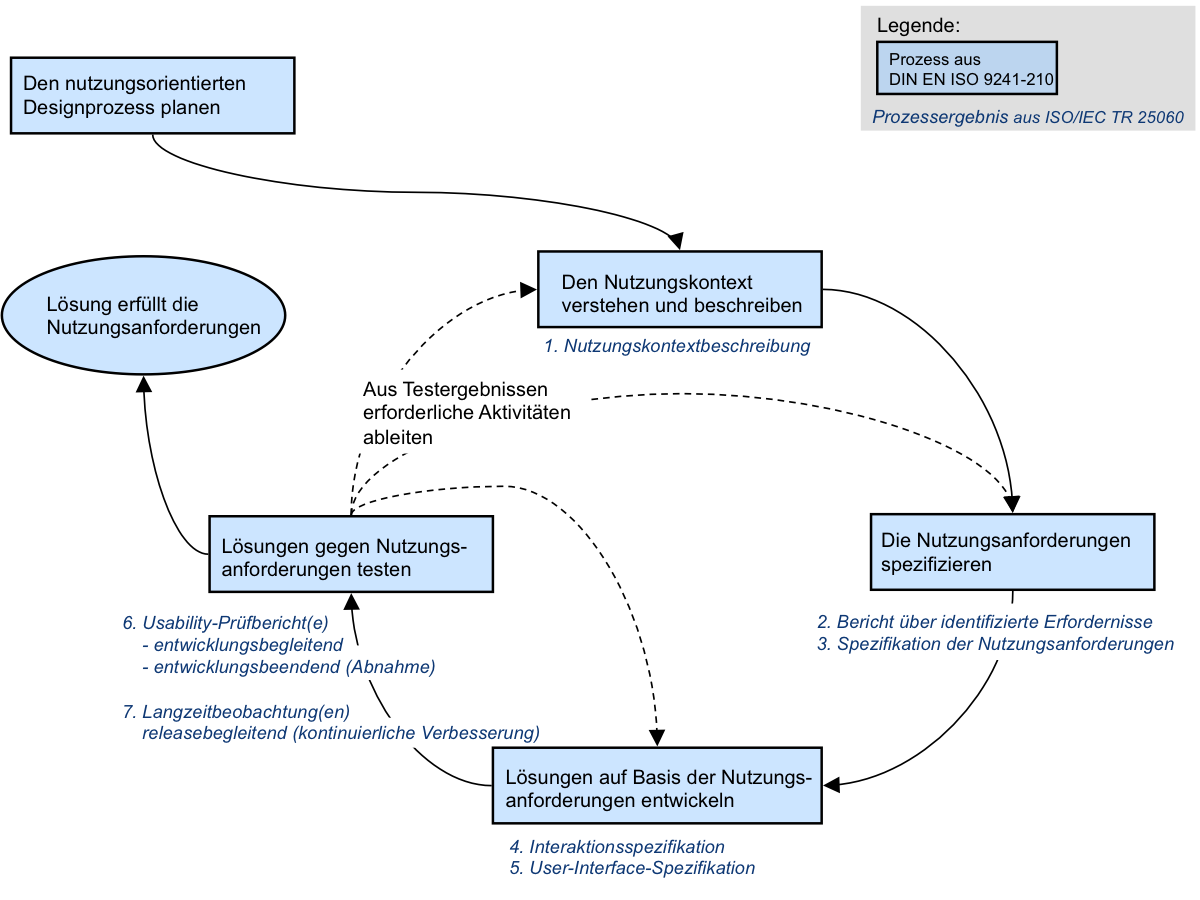
\includegraphics[width=.9\textwidth]{./images/prozessergebnisse.png}
\caption{Prozessmodell menschzentrierter Gestaltung nach ISO 9241-210 }
\label{prozessmodell}
\end{figure}

Wie bereits der Bezeichnung zu entnehmen ist, konzentriert sich dieser Ansatz auf die Fokusierung des Benutzers und seine Eigenschaften und wird in mehreren Prozessphasen stetig validiert und überarbeitet. Nach der Planung des Gestaltungsprozesses erfolgt in diesem Modell die Auseinandersetzung mit dem Nutzungskontext und der Anforderungen. Für das Projekt wäre eine dahingehende Untersuchung sinnvoll, um zu Beginn ein umfangreiches Bild über die Benutzer, ihre Motivationen und den Anwendungsbereich zu gewinnen. 
Der menschzentrierte Gestaltungsprozess setzt dabei stark auf die Zusammenarbeit mit den Benutzer und versucht eine Gestaltungslösung zu erarbeiten, die an ihre speziellen Bedürfnisse angepasst ist. Dieses Vorgehen eignet sich dann besonders gut, wenn man seine Nutzer kennt und diese konkret ausmachen kann. In Anbetracht der Problemdomäne, ist dieser Ansatz jedoch nicht ganz so leicht zu realisieren. Prinzipiell kann jeder Mensch die Anwendung benutzen, sofern er dazu eine Motivation aufbringt. Sie verfolgen dabei alle das selbe Ziel, können jedoch aus unterschiedlichsten Bereichen stammen und verschiedene Fähigkeiten und Eigenschaften aufweisen. Daher lässt sich ein Fokus auf die Menschen hierbei nicht angemessen realisieren. Was an diesem Modell für das Entwicklungsprojekt zweckmäßig erscheint, ist der iterative Prozesscharakter (bis zu einem gewissen Rahmen) und der anfängliche Fokus auf Nutzungskontext und Anforderungen .\\
Neben dem User centered Design, gibt es einen weiteren Ansatz der MCI. Geprägt ist dieser durch Larry Constantine und Lucy Lockwood und wird als usage-centered Design. Dieses Vorgehensmodell legt dabei den Fokus auf die Interaktion zwischen den Anwendern und den funktionalen Aspekten des Systems. Prinzipiell soll hierbei die Gebrauchstauglichkeit eines Systems verbessert werden und an die user needs ausgelegt werden. \\
Nach Betrachtung der beiden Ansätze, wurde entschlossen mit Methoden des usage centered Design zu arbeiten, da der Problemfokus nicht direkt auf den Benutzern liegt, sondern vorallem auf den Aktivitäten die diese durchführen um ihr Ziel zu erreichen. Gerade die Kommunikation der Anwender untereinander ist wesentlicher Bestandteil des Konzeptes. Anfänglich soll demnach eine Kombination beider Vorgehensmodelle verwendet werden, sodass eine gründliche Auseinandersetzung mit den möglichen Anwendern Anhaltspunkte für die Interaktionen liefern kann. Stakeholdermodellierung und die Erstellung von User Profiles identifizierter Gruppen wäre hierbei ein erster Schritt\footnote{Informationen über http://www.foruse.com/questions/index.htm\#13 und ISO 9241-210}. 

\newpage

%!TEX root = ../Dokumentation.tex


\section{Projektbezogenes XML Schemata}

\subsection{Vertiefung}
Der erste Meilenstein befasst sich mit der Repräsentation von Daten in XML.\\

Damit bei der Verwendung der XML Dateien bei der späteren Verarbeitung mit JAXB keine Probleme auftreten, ist es notwendig eine Validierung der Dateien durch Definition zugehöriger XML Schemas durchzuführen. Vorteil bei der Verwendung eines Schemas ist, neben der Kontrolle auf Wohlgeformtheit und der Verwendung definierter Datentypen und Strukturen, auch das festlegen von Restriktionen.\\

Hinsichtlich des zugrunde liegenden Konzeptes und den benötigten Informationen, gibt es viele Elemente innerhalb der Dateien, die nur mit Strings realisiert werden können. Das Problem bei freier Definition
besteht darin, dass die Datensätze sehr fehleranfällig sind, wenn es um die Benutzung durch Menschen geht. Rechtschreibfehler beim Namen des Landes, des Fernsehsenders oder des Genres, würden für den Benutzer der Anwendung noch kein Problem darstellen, da er vermutlich deuten könnte was gemeint ist. Für die Umsetzung ist es aber von Vorteil, die Datensätze möglichst konsistent zu halten.\\

Das System des Serientrackers beruht darauf, die Verwaltung von Serien anhand von Listen zu ermöglichen. Wie bereits in der Besprechung der Umsetzung erwähnt, wird anhand dieser Informationen auch die asynchrone Datenübertragung realisiert.\\
Das Abonnieren von Informationen zu laufenden Serien des Genre Action, greift bei Benachrichtigung auf Datensätze zu, die diesem Elementwert unter dieser eindeutigen Zeichenfolge zugeordnet sind. Formulierungsfehler wie \textit{Aktion}, die von einer einheitlichen Schreibweise abweichen, führen dementsprechend zu Komplikationen, weil sie die Konsistenz der Informationssätze beschädigen.\\

\vspace{0.2cm}

Hinsichtlich des Themas Serien, führten die Vorüberlegungen zu dem Entschluss, dass folgende Objekttypen innerhalb des Serientrackers von interesse sind und wiederkehrende Elemente darstellen:\\

\vspace{0.2cm}

\textbf{Serie}\\
Eines der wichtigsten Elemente, dass alle Informationen beinhaltet, die für den Benutzer von bedeutung sind, ist die Serie. Eine Serie besitzt allgemeine Informationen wie Name, eine Beschreibung, der Sender auf dem sie ausgestrahlt wird oder das Produktionsland. Im realen Kontext wird eine Serie zudem in Seasons (Staffeln) ausgestrahlt, die jeweils eine bestimmte Anzahl von Episoden enthalten.

\vspace{0.2cm}

\textbf{Season}\\
Bestandteil einer Serie, von der es im Laufe der Jahre immer neue Objekte gibt und die nach einer gewissen Anzahl an Episoden als abgeschlossen gelten.

\vspace{0.2cm}

\textbf{Episode} \\
Ein Kernelement des Systems, dass ein wichtigen Typ für die asynchrone Kommunikation darstellt. Durch das Abonnieren von Genres oder Serien, wird die Benachrichtigung in Bezug auf eine einzelne Episode ausgelöst, die sich durch ihr jeweiliges Austrahlungsdatum und -zeitpunkt kennzeichnet. Zudem kann der Inhalt der Episode von Interesse sein.

\vspace{0.2cm}

\textbf{User}\\
Neben den Serieninformation, gibt es die Benutzer des Serientrackers, die sich anmelden und durch Listen die Dienste des Serientrackers abonnieren.
Allgemein werden hierbei personenbezogene Daten wie Username und echter Name erwartet, so wie Zusatzinformationen, die für andere Benutzer von Interesse sein könnten und die Person hinter dem Profil genauer beschreiben. Beispiele wären das Alter, ein Profilbild, Wohnort oder eine kurze Beschreibung.

\vspace{0.2cm}

\textbf{Liste}\\
Die Liste kann als Sammlung mehrerer Serien zu einem bestimmten Thema aufgefasst werden. Hierbei gibt zum einen Listentypen die definitiv vorhanden sein müssen, wie beispielsweise Genrelisten oder die Favoritenliste eines Benutzers. Diese erfasst die Serien, zu denen der Eigentümer Benachrichtigungen erhalten will. Zum anderen besteht aber auch die Möglichkeit, dass der Benutzer sich Listen anlegt, die seinen individuellen Wünschen entsprechen.

\vspace{0.2cm}

\textbf{Message}\\
Als zusätzlicher Typ, der jedoch erst in der asynchronen Kommunikation verwendung finden wird, wurde die Message identifiziert. Hierbei handelt es sich um eine bestimmte Nachricht, die den entsprechenden Usern bei Eintreten eines Events zugeschickt wird und ein neues Ereignis meldet.


\newpage

\subsection{Realisierung der Schemata}

Nach der theoretischen Planung fand die Realisierung der XML Schemata statt.
Dabei wurde für jeden der zuvor identifizierten Obertypen ein eigenes Schema definiert und die einzelnen Elemente/Attribute mit Datentypen und Restriktionen belegt. Die Aufteilung der einzelnen Typen auf ein seperates Schema, fand mit den Gedanken statt, die Struktur der Daten möglichst einfach und lesbar zu halten. Eine Serie die mehrere Staffeln enthält, die wiederrum jeweils eine Menge von Episoden auffassen, würde ein sehr komplexes Element definieren, dass während der Entwicklung schnell zu unübersichtlich werden kann.\\

Da die Daten einer Episode, inhaltlich jedoch weiterhin davon abhängen, von welcher Serie diese ist und in welcher Staffel sie vorkam, wird eine Referenzierung mit Hilfe von global eindeutigen IDs eingeführt. Jede Serie, User, Season, Episode, Message und Liste wird mit einer einzigartigen Folge von Zeichen beschrieben, über diese es möglich ist auf gewünschte Informationen zuzugreifen und entsprechende Elemente auszulesen.\\

Dieses Prinzip lässt sich am Beispiel des XML Schemas einer Episode veranschaulichen. Hierbei handelt es sich um einen Codeauszug, der die gesamte Struktur einer Episode vorgibt:\\

\begin{lstlisting}[basicstyle=\ttfamily,numbers=left,numberstyle=\footnotesize\ttfamily,backgroundcolor=\color{source},basicstyle=\ttfamily,numbers=left,numberstyle=\footnotesize\ttfamily,backgroundcolor=\color{source},label=xsd-definition-episode,caption= Definition des complexElement Episode mit Elementen und Attributen]
  <xs:element name="episode">
    <xs:complexType>
      <xs:choice minOccurs="0">
        <xs:sequence>
          <xs:element ref="episodeNumber"/>
          <xs:element ref="title"/>
          <xs:element ref="overview"/>
          <xs:element ref="airdate"/>
          <xs:element ref="images"/>
        </xs:sequence>
      </xs:choice>

      <xs:attribute ref="serieID" use="required"/>
      <xs:attribute ref="seasonID" use="required"/>
      <xs:attribute ref="episodeID" use="required"/>
    </xs:complexType>
  </xs:element>
\end{lstlisting}

Eine Episode bekommt damit eine eindeutige \textbf{episodeID} zugeordnet und ist, gesehen unter allen Episoden, eindeutig identifiziert. Zudem erhält jede Episode auch die Referenz der serienID und seasonID als Attribute, um Verweise und Zuordnungen zu realisieren. Da sich jedes Objekt demnach durch eine Kennung repräsentiert, reicht bei anlegen von Listen und Containern ein einfacher Verweis auf entsprechendes Element, wodurch Datenredundanz bei mehreren Schemata verhindert wird, die inhaltlich voneinander abhängen. Innerhalb der XML Datei einer Serie, reicht somit der Verweis auf die einzelnen Seasons über ihre ID, ohne dass deren Inhalte mehrfach abgespeichert werden müssen. Dieser Redundanzverlust wäre auch realisierbar gewesen, wäre eine Season und Episode direkt innerhalb des Serieschemas gespeichert worden. Damit hätte eine Referenz auf die Serie genügt und auf eine Episode könnte mit einer Abfrage der Seasonnummer und Episodennummer getätigt werden. Der Entschluss zur Aufteilung der Schemata führte jedoch zwangsläufig zu dieser Entscheidung, wobei die Folge daraus auch komfortable Vorzüge in der Flexibilität der einzelnen Elemente mit sich bringt.\\
Um die Struktur des gesamten Serien Elements zu ermöglichen und vorhandene IDs global nutzen zu können, wird jedes Schema über eine Masterdatei in die einzelnen XML Schemas inkludiert, um bereits definierte Elemente und Attribute wiederverwendbar zu machen und die Datenmenge zu reduzieren.

\begin{lstlisting}[basicstyle=\ttfamily,numbers=left,numberstyle=\footnotesize\ttfamily,backgroundcolor=\color{source},label=xsd-definition-master,caption= Auszug aus der Masterinklude Serientracker.xsd]
<!-- Dieses Schema inkludiert alle zu verwendenen Schemata-->

<xs:schema xmlns:xs="http://www.w3.org/2001/XMLSchema">

  <xs:include schemaLocation="Series.xsd"/>
  <xs:include schemaLocation="Serie.xsd"/>
  <xs:include schemaLocation="Seasons.xsd"/>
  <xs:include schemaLocation="Season.xsd"/>
  <xs:include schemaLocation="Episodes.xsd"/>
  <xs:include schemaLocation="Episode.xsd"/>

  <xs:include schemaLocation="Lists.xsd"/>
  <xs:include schemaLocation="List.xsd"/>
  <xs:include schemaLocation="Users.xsd"/>
  <xs:include schemaLocation="User.xsd"/>
  <xs:include schemaLocation="Message.xsd"/>

  <!-- Globale Elemente -->
\end{lstlisting}

Neben dem Include der einzelnen Schemata, werden auch vereinzelte Elemente darin definiert, die innerhalb der einzelnen Schemata wiederholt Verwendung finden. Hierbei vor allem die einzelnen ID Attribute.\\

Während der Entwicklung dieser Variante, gab es anfängliche Schwierigkeiten innerhalb der Umsetzung. Der Verweis innerhalb eines XML Schemas auf ein Anderes und die entsprechende Verwendung der Elemente und Attribute, führte zu Komplikationen innerhalb der Deklarationen. Auch eine Definition eines einheitlichen Namespaces führte zu keiner Lösung. Im zweiten Ansatz folgte dann die direkte Auseinandersetzung zwischen den Optionen Include und Import, wobei die letztendliche Wahl auf die Inkludierung fiel. Ein Import erlaubt den Verweis auf unterschiedliche Namespaces, wobei ein Include auf einen einheitlichen Namespace verweist und bei nichtbestehen, den des Oberschemas übernimmt.\\
Da Namespaces in der Regel dazu dienen, Elementen und Attributen einen gewissen Namensraum zu gewährleisten, der bei gängigen Bezeichnungen wie \textit{Name} zu Konflikten führen kann, ist die Definition bei größeren Projekten durchaus zu empfehlen. Ob dabei ein Einzelner oder Mehrere angelegt werden sollten, ist eventuell auch abhängig von der gesamten Struktur des Schemas. Da im Rahmen dieses Projektes jedoch mit relativ geringem Datenumfang gearbeitet wird und mit keiner Komplikation der Bezeichnungen zu rechnen ist, wurde auf eine genaue targetNamespace Definition verzichtet. Auch wenn bestimmte Elementbezeichnungen innerhalb eines \textit{http://Serientracker.de} Namensraum denkbar gewesen wäre. Letztendlich spielt dieser Aspekt für die Umsetzung innerhalb des Projektes jedoch keine tragenden Rolle. Daher wurde auf die Definition verzichtet und die entsprechende Include Variante verwendet.

\vspace{0.2cm}

Ein weiterer Punkt der in der Entwicklungsphase von Bedeutung war, war die Frage danach, wie die Daten innerhalb des lokalen Speichers abgelegt werden.
Durch die Definition einzelner Schemas erhält jedes Objekt dieses Typs auch eine eigene XML Datei. Im späteren Verlauf könnten sich daraus aber Probleme beim gezielten Zugriff entwickeln, denen frühzeitig Abhilfe geschaffen werden sollte.\\
Aus diesem Grund wurde eine weitere Gruppe von Elementen innerhalb XML angelegt, die Containerklassen.\\
Für jeden Elementtyp, der als eigene Entität angelegt wird, wurde eine Containerklasse definiert, innerhalb derer beliebig viele Objekte eines bestimmten Typs aufgenommen werden können. Dieses Objekt dient in der letztendlichen Verwaltung als Sammlung aller Elemente.\\

\newpage
Folgendes Beispiel veranschaulicht den Ansatz und wurde in dieser Form für jeden Elementtyp angelegt:
\begin{lstlisting}[basicstyle=\ttfamily,numbers=left,numberstyle=\footnotesize\ttfamily,backgroundcolor=\color{source},label=xsd-definition-series,caption= Auszug aus der Series.xsd Definition]
<!-- Element das alle Serien aufnimmt -->
  <xs:element name="series">
    <xs:complexType>
      <xs:sequence>
        <xs:element ref="serie" minOccurs="0" maxOccurs="unbounded"/>
      </xs:sequence>
    </xs:complexType>
  </xs:element>
\end{lstlisting}


Um die vorhandenen Daten semantisch sinnvoll und reichhaltig anzulegen, wurde bei der Entwicklung der XML Schemata darauf geachtet, diesen Anspruch
durch die verschiedenen Datentypen, Restriktionen und Benutzungstypen zu gewährleisten.

\subsection{Datentypen}

Grundsätzlich werden innerhalb des Serientrackers Daten unterschiedlichen Typs benutzt, die entsprechend des realen Kontextes am sinnvollsten erscheinen.
Aufgrund der Komplexität, soll hierbei nicht auf jedes einzelne Element eingegangen werden, sondern nur ein Überblick darüber vermittelt werden, mit welchen Grundideen vorgegangen wurde.

\vspace{0.2cm}

Neben den einfachen Standartdatentypen wie String, Boolean, Integer, Time (...), bietet XML die Möglichkeit weitere spezifische Typen wie anyURI oder ID zu definieren.\\
Da innerhalb des Serientrackers viele Information lediglich in Textform sinnvoll sind, wurde für diese der Typ \textbf{String} verwendet. Beispielhaft seien hier die Titel und Beschreibungen, sowie Benutzernamen und Länder erwähnt.\\
Jahreszahlen, Episodenlänge und Season- und Episodennummern werden mit Zahlen als \textbf{Integer} ausgedrückt. Bestimmte Zeitangaben wie Ausstrahlungszeit, bei denen es nur um den Zeitpunkt geht, in der einfach Form \textbf{Time} und genauere Angaben, wie bei Ausstrahlungstag in Hinsicht auf die Benachrichtigung, über den \textbf{dateTime} Typ.
Linkverweise auf Bildquellen wie bei Avatar erhielten den Typ \textbf{anyURI}.\\

\vspace{0.2cm}

Einzelne Elemente wie User und List, weisen hierbei noch eine Besonderheit auf. Wie bereits bei den Kommunikationsabläufen innerhalb des Konzepts angesprochen, wird die Anwendung von Benutzern verwendet, die verschiedenen Rechtetypen angehören.\\ Aus diesem Grund wird jeder User mit dem Attribute Admin gekennzeichnet, der innerhalb einer einfachen \textbf{Boolvariablen} die entsprechenden Rechte festgelegt. Ähnliches Prinzip wird bei den Listen verwenden zur Unterscheidung, ob die Sichtbarkeit für jeden Benutzer gestattet ist oder nur für den Besitzer der Liste.

\vspace{0.2cm}

Zur angesprochenen Referenzierung und Identifizierung einzelner Entitäten, zeichnen sie sich durch eine eindeutige ID als Attribut aus. Generell wurden die Informationen wie ID oder Rechte, die ein Objekt nicht inhaltlich sondern eher aus verwaltender Sicht genauer beschreiben, als Attribute definiert. Inhaltliche Informationen die Bestandeteil des Objektes sind, werden hingegen als Elemente angelegt.\\

Für den Datentyp einer solchen ID, wurde ein eigenes Element folgendermaßen definiert:
\begin{lstlisting}[basicstyle=\ttfamily,numbers=left,numberstyle=\footnotesize\ttfamily,backgroundcolor=\color{source},label=xsd-definition-idtype,caption= Definition der globalen IDs]
  <xs:simpleType name="idType">
    <xs:restriction base="xs:string">
      <xs:pattern value="|(ss|sn|ep|us|ls|me)_[0-9a-z]{8}"/>
    </xs:restriction>
  </xs:simpleType>
\end{lstlisting}

Am Anfang der Zeichenketten steht ein Kürzel, dass den jeweiligen Typ angibt. SN steht dabei für Season, EP für Episode und ähnliches. Danach folgt ein optisches Trennzeichen, gefolgt von einer beliebigen Characterfolge aus 8 gemischten Zeichen mit Zahlen und Buchstaben. Eine Serie erhält damit eine Zuordnung der Form \textit{ss\_0a1b2c3d}.


\subsection{Restriktionen}
Damit die Informationen innerhalb der XML Dateien inhaltlich sinnvoll sind und während der Verarbeitung keine weiteren Probleme entstehen (zum Beispiel durch unterschiedliche Schreibweisen), wurden für einige Elemente Restriktionen definiert.\\
Dabei ist das Ziel, die Fehleranfälligkeit zu reduzieren und im Kontext logische Informationen zu gewährleisten. Vorhandene Restriktionen, also Einschränkungen/Bedingungen, die für einzelne Elemente getroffen wurden, sind im folgenden mit einer kurzen Begründung aufgeführt. Häufig treten diese in Form von Längenbegrenzungen bei Texten auf oder als Grenzbereichen bei Zahlen.\\
Weitere Elemente kennzeichnen sich entsprechend dadurch, dass der Inhalt auf eine bestimmte Auswahl an Möglichkeiten eingeschränkt wurde. Beim Konzipieren dieser Grenzen und Auswahlmöglichkeiten, ist es nicht möglich die perfekte Variante zu erzielen, sondern eine Auswahl von Optionen zu treffen, die im Kontext als zuverlässig und praktikabel erscheinen. Manche Begrenzugnen wie Anzahl an Episoden einer Staffel oder Episodenlaufzeit, wurden in Bezug auf die Realität getroffen und angelehnt an gängige Formen. Prinzipiell wären hierbei alternative Auswahlmöglichkeiten und Varianten denkbar, wie beispielsweise die freie Definition des Genres oder des TV Senders als einfacher String. Hierbei hat der verwaltende Admin dann die Option den Inhalt frei zu bestimmen. Letztendlich wurde jedoch der eigentliche Nutzen abgewägt, sodass für den Serientracker folgende Restriktionen definiert wurden:

\begin{table}[H]
\caption{Allgemeine Restriktionen}

\begin{tabular}{l l l}
\\ [-0.5ex]

\hline\hline
\\ [-0.5ex]
Element/Attribut & Restriktion & Begründung
\\ [1.5ex]
\hline
\\ [-0.5ex]
Overview (global) & Stringlänge 10 < und < 500 & allgemeinen Informationen,\\[1ex]
&&kurze Inhaltsangabe\\[3ex]
Title (global) & Stringlänge 1 < und < 80 & gängige Titellänge\\[3ex]
Name (list) & Stringlänge 2 < und < 80 & treffende Bezeichnung,\\[1ex]
&&Name keine Beschreibung \\[3ex]
Public (list) & Boolean True und False & feste Zustände \\[3ex]
Episodenumber (episode) & Anzahl < 26 & sinnvolle maximale Episodenanzahl\\[3ex]
Seasonnumber (seasons) & Anzahl < 41 & sinnvolle Begrenzung, \\[1ex]
&&Freiraum für Langzeitserien \\[2ex]

\hline
\end{tabular}
\label{tab:restriktionenderxsdgeneral}
\end{table}


\begin{table}[H]
\caption{Restriktionen des User Schemas}
\centering

\begin{tabular}{l l l}
\\ [-0.5ex]

\hline\hline
\\ [-0.5ex]
Element & Restriktion & Begründung
\\ [1.5ex]
\hline
\\ [-0.5ex]
Username & Stringlänge 2 < und < 30 & sinnvolle Namenlänge,\\[1ex]
&& verhindert Text \\[3ex]

Lastname & Stringlänge 1 < und < 40 & gängige Nachnamenlänge, \\[1ex]
&&eventuell Doppelnamen,\\[1ex]
&&verhindert Text \\[3ex]

Firstname & Stringlänge 1 < und < 50 & gängige Vornamenlänge, \\[1ex]
&&Mehrfachnahmen \\[3ex]

Gender & Auswahl zwischen Male und Female & logische Auswahl, \\[1ex]
&&Vorgabe verhindert Schreibfehler\\[3ex]

Age & älter als 13 und jünger als 121 & Mindestalter zur Nutzung, \\[1ex]
&&logische Obergrenze \\[3ex]

Location & Stringlänge < 40 & Stadtname, Land etc. \\[1ex]
&&Eingabe ist keine Adresse\\[1ex]
&&und lässt sich in Kürze ausdrücken\\[3ex]

About & Stringlänge < 200 & optionale Kurzbeschreibung,\\[1ex]
&&nach oben begrenzt, \\[1ex]
&&zu viele Informationen nicht \\[1ex]
&&unbedingt von Interesse  \\[3ex]

Admin & Boolean ob True or False & Rechtevergabe nach Status,\\[1ex]
&&Auswahl nur in 2 Zuständen möglich\\[2ex]

\hline
\end{tabular}
\label{tab:restriktionenderxsduser}
\end{table}


\begin{table}[H]
\caption{Restriktionen des Serie Schemas}


\begin{tabular}{l l l}
\\ [-0.5ex]

\hline\hline
\\ [-0.5ex]
Element & Restriktion & Begründung
\\ [1.5ex]
\hline
\\ [-0.5ex]
Year & Jahreszahl 1900 < und < 2015 & Jahreszeiten außerhalb\\[1ex]
&&unrelevant \\[3ex]

Country & Auswahlmöglichkeit Ländern & Eingabefehler verhindern\\[3ex]
Episoderuntime & Auswahl zwischen gängigen Episodenlängen& Serie hat feste Episodenlänge\\[3ex]
Network & Auswahl bekannter Sender & unrelevante Sender entfallen,\\[3ex]
&&Eingabefehler verhindern\\[3ex]

Airday & Auswahl des Tagnamen & Eingabefehler verhindern\\[3ex]
Genre & Auswahl definierter Genres & einheitliche Schreibweise,\\[1ex]
&&Eingabefehler verhindern,\\[1ex]
&& sinnvolle Genre\\[2ex]

\hline
\end{tabular}
\label{tab:restriktionenderxsdserie}
\end{table}



\subsection{Beispieldaten}

Bereits während der Entwicklung der XML Schemas, wurden parallel XML Dateien mit entsprechenden Beispieldaten definiert. Durch den entsprechenden Validierungstest bietet sich zum einen die Möglichkeit entsprechenden Definitionen auf Korrektheit zu prüfen und zum anderen XML Typen zu entwickeln, die möglichst praxistaugliche Elemente und Attribute aufweisen. Zu jedem XML Schema wurde daher mindestens eine Beispieldatei erzeugt und die entsprechende Referenzierung untereinander getest. Speziell im Containerelemente Series wurde deutlich, wie flexibel die Datensicherung mit globalen IDs sein kann. Zum einen reicht das Einbinden eines Objekts in der simplen Form <serie serieID="ss\_6127hdja"/>, zum anderen kann auch die gesamte Struktur einer Serie inklusive Informationen über Season und die einzelnen Episoden eingebunden werden.\\

\vspace{0.2cm}

Für die entsprechende Nutzung in der weiteren Entwicklung, wurden zudem korrekte Beispieldatensätze von Serien angelegt. Diese Repräsentieren von der obersten Ebene der allgemeinen Serieninformationen bis hin zur niedrigsten Ebene der einzelnen Episodeninformation vollständige Datensätze, wie sie in einem komplexen System dieser Form angelegt werden müssten. Aufgrund von Testzwecken, wurde sich jedoch auf wenige Beispielserien beschränkt. Zudem wurden entsprechende Daten innerhalb der Series.xml definiert und nicht in die entsprechenden Typen aufgeteilt. Diese Variante hatte zum Vorteil, dass die Informationen einer Serie (für Menschen) übersichtlich strukturiert und lesbarer waren, als wenn jede Beispielepisode per Hand in einzelne XML Files getrennt worden wäre.
Aufgrund der Vielzahl von Informationen zeigte, sich aber bereits bei wenigen Daten der Nachteil, dass die Datei sehr komplex wurde. Darüber hinaus weist diese Variante auch die Schwäche beim möglichen Datenverlust auf. Sollte in diesem Fall das sammelnde Element verloren gehen, so wäre der Datenverlust größer gegenüber den seperaten Absicherungen in einzelnen Files.

\vspace{0.2cm}

In der Konzeptvorstellung wurde von der möglichen Einbindung einer Freundefunktion gesprochen. Die Umsetzung dieses Themas würde noch eine Änderung der XML Schemata der User mit sich ziehen. Ähnlich wie für die Abonnements von Serien, könnte man innerhalb des User Schemas ein komplexes Element \textit{Friends} einbauen, dass beliebig viele User aufnimmt. Dabei könnten normale Objekte des bereits vorhandenen Userschemas eingebunden werden und eine Liste aller Freunde bilden.\\ Um die entsprechende Kommunikation zwischen den einzelnen Freunden zu gewährleisten und Meldungen wie Empfehlungen oder Benachrichtigungen zu verschicken, muss weiterhin das Message Schema erweitert oder alternativ ein neues Schema der \textit{Friendmessage} eingeführt werden. Eine seperate Trennung beider Nachrichtenarten wäre in sofern sinnvoll, als das diese in der Funktionalität und Definition unterschiedliche Anwendungen haben. Die bisherigen Nachrichten werden von der Serverseite aus an User geschickt und beinhalten statische Nachrichten. Auch Empfehlungen könnte man mit festen Standartnachrichten wie \textit{X empfiehlt dir Serie Y} umsetzen, jedoch wäre hierbei in der Regel eine persönlichere Komponente wie Userkommentare mit enthalten.

\vspace{0.2cm}

Sofern dieser Aspekt umgesetzt wird, müsste man hierbei die entsprechenden Varianten abwägen und dabei mögliche Szenarien konzeptionell durchspielen, um eine passende Einbindung hinsichtlich der Funktionalität zu finden.\\
Nach der Auseinandersetzung mit den vorhandenen Daten und entsprechender Definition der XML Schemas, folgt im nächsten Schritt die Entwicklung der synchronen Kommunikationskomponenten.


\newpage

%!TEX root = ../Dokumentation.tex

\section{Ressourcen und die Semantik der HTTP-Operationen}
\subsection{Vertiefung}

Als Vorbereitung für die Umsetzung der synchronen Kommunikationsvorgänge, steht die theoretische Auseinandersetzung mit REST im Mittelpunkt.
Der erste Schwerpunkt dabei ist die Identifizierung vorhanderer Ressourcen des Serientrackers. Bereits beim Konzipieren der XML Schemas mit beispielhaften XML Datensätzen, musste überlegt werden, für welche Elemente es möglich ist Entitäten der realen Welt zu ermitteln.\\

Bei einer Ressource geht es, ähnlich wie bei XML Dateien, nicht darum wie die darin enthalten Informationen im letztendlichen Kontext repräsentiert werden, sondern welche Informationen diese enthalten. Entsprechende Objekte der Außenwelt werden beschrieben und wie die Wurzelelemente bei XML, stellen sie einen bestimmten Objekttyp dar. Eine identifizierte Ressource, ist eine Schnittstelle zur Außenwelt und sollte daher dem Kontext entsprechend gut durchdacht werden.\\
Die Auseinandersetzung mit den XML Schemas lieferte dabei einen Überblick über vorhandene Primärressourcen. Dabei handelt es sich um die Oberklassen der vorhandenen Objekttypen \textit{Serie} und \textit{User}.\\

Desweiteren ist es möglich vorhandene Subressourcen zu identifizieren, die sich dadurch auszeichnen, dass sie selbst Bestandteil einer Ressource sind.
Aufgrund der komplexen Struktur einer Serie, die neben den allgemeinen Informationen noch die Informationen zu mehreren Staffeln und entsprechenden Episoden enthalten, wurde früh die systematische Aufteilung festgelegt.
Da es auch innerhalb der Anwendung von Interesse sein kann, eine einfache Repräsentation der Staffelübersicht oder der Episodenübersicht einer Staffel zu ermöglichen, bietet es sich gerade bei diesen Typen an, diese Objekte als eigene Ressource zu designen. Dazu kommt, dass eine Episode zum Beispiel im Kontext einer Serie am meisten Sinn macht, durchaus aber auch für sich existieren kann. Zur Ordnung der einzelnen Elemente, gibt es entsprechende Listenressourcen wie Series, Seasons, Users und Episodes, welche alle Elemente des zugehörigen Typs aufnehmen und sammeln.\\

Ein Kernelement der Anwendung wird das Benachrichtigen der Benutzer über bestimmte Ereignisse sein. Diese Abonnements lassen sich in Listen verwalten. Gerade bei einer möglichen Kategorisierung wie beispielsweise \textit{Serie mit dem Genre Drama}, wäre es durchaus interessant gewesen Listenressourcen mit entsprechenden Filtern zu definieren. Aufgrund der Vielzahl von Kategorisierungsmöglichkeiten, wird dieser Schritt aber nicht über einzelne Ressourcen stattfinden, sondern innerhalb der Anwendung durch die Abfrage bestimmter Elemente erzielt.\\

\vspace{0.2cm}

Die theoretische Auseinandersetzung führte zu folgenden Ressourcen, wobei die angegeben URI nur den charakteristischen Abschnitt widerspiegelt.
Da für die Umsetzung an sich, die URI eher als eine ID in Form von Zeichen steht und für die letzendliche Auswertung keine semantische Korrektheit notwendig ist, wird auf eine Darstellung in Form mit Schema und Pfadangabe in der Übersicht verzichtet.

\begin{table}[H]
\caption{Ressourcen des Serientrackers}

\centering
\begin{tabular}{l l l}
\\ [-0.5ex]

\hline\hline
\\ [-0.5ex]
Ressource & URI & Methode
\\ [1.5ex]
\hline
\\ [-0.5ex]
Liste aller Serien & /series/ & GET, POST \\[1ex]
Einzelne Serie & /series/\{id\} & GET, PUT, DELETE\\[1ex]
Liste aller Staffeln & /seasons/ & GET, POST \\[1ex]
Einzelne Staffel & /seasons/\{id\} & GET, PUT, DELETE\\[1ex]
Liste aller Episoden & /episodes/ & GET, POST \\[1ex]
Einzelne Episode & /episodes/\{id\} & GET, PUT, DELETE\\[1ex]
Liste aller User & /users/ & GET, POST \\[1ex]
Einzelne User & /users/\{id\} & GET, PUT, DELETE\\[1ex]
Liste aller Listen & /lists/ & GET, POST\\[1ex]
Liste eines Users & /lists/\{id\} & GET, PUT, DELETE\\[1ex]
\hline
\end{tabular}
\label{tab:ressourcendesserientrackers}
\end{table}

Jedes Element, dass für die synchrone Kommunikation von Interesse ist, besitzt eine Ressource als einzelnes Element\\
(Form:/ressourcenname/\{id\}) und die Gesamtheit einer Liste (Form:/ressourcenname/). Bei den URI wird der Zugriff über entsprechende ID's auf die Liste deutlich und es zeigt sich eine Folge der einfachen URI. Durch die Konzipierung der Untertypen Staffel und Episode als einzelne Ressource, ist eine entsprechender Aufruf auf das bestimmte Element möglich.\\
Vorstellbar aufgrund der allgemeinen Struktur wäre auch ein Pfad der \\
Form /series/\{id\}/seasons/\{id\}/episodes/\{id\}.  Dieser setzt entsprechend vorraus, dass nicht nur die einfache Episoden ID, sondern auch die zugehörige Serien ID und Season ID bekannt ist.

\subsection{Semantik der HTTP-Operationen}

Nachdem die Ressourcen identifiziert sind, muss nun bestimmt werden, welche Operationen (HTTP-Methoden) unterstützt werden und welche Semantik sich dahinter verbirgt.\\
Dafür stehen die vier Methoden GET (Informationen auslesen), POST (Informationen anlegen), PUT (Informationen ändern) und DELETE (Informationen löschen) zur Verfügung. Nicht jede Ressource muss alle Methoden bereitstellen. Für das Projekt wurden die Ressourcen erneut betrachtet und die benötigten Methoden samt Semantik herausgearbeitet. Dabei entwickelte sich folgende Ergebnis:

\begin{figure}[H]
\includegraphics[width=.9\textwidth]{../images/bedeutunghttpmethoden.png}
\caption{Bedeutung der http Methoden}
\label{bedeutunghttpmethoden}
\end{figure}


\newpage

%!TEX root = ../konzept.tex

\section{Nutzungskontext}
Nach der Betrachtung der vorhandenen Benutzer, folgt nun ein erster Grobriss des Nutzungskontext\footnote{Nach Inhalt der ISO 9241-210, Prof. Hartmann Draft zur MCI ab S. 544}.\\
Dabei sollen wesentliche Eigenschaften der potentiellen Benutzer eingeschätzt und der Betrachtungsraum auf Arbeitsmittel, das physikalische Umfeld und Ziele erweitert werden.\\


Benutzer
\begin{itemize}
   \item 
   Altersklassen: Nicht exakt definierbar, grundsätzlich jeder der ein Smartphone besitzt und auf diese Art und Weise Reisen will. Kernzielgruppe wird zwischen 16 - 50 Jahre geschätzt. Prinzipiell könnten auch Personen darüber hinaus Interesse an der Applikation haben. Vorraussetzung ist lediglich die vorhandene Technologie. Vermutlich spricht der sozialere Aspekt diese aber eher weniger an und sind wahrscheinlich nicht mit Campingausrüstung längere Zeit unterwegs. Physische Merkmale befähigen sie als Mieter dazu, eine Reise aufzunehmen. Als Vermieter gibt es dahingehend keine Einschränkung.

   \item 
   Einkommen: Grundsätzlich sind Personen aller Einkommensklassen möglich. Aufgrund des Kostenfaktors wird die Kernzielgruppe jedoch hauptsächlich aus einer einkommensschwächeren oder besonders finanzbewusste Schicht stammen.

   \item 
   Erfahrung der Benutzer: Mit Erfahrung der Campingdomäne kann gerechnet werden, muss aber nicht zwangsläufig vorhanden sein.
   Erfahrene Leute in diesem Bereich, haben eventuell schon einige Apps ausprobiert und in Benutzung und können mit solchen Systemen sicher umgehen.
   Grundsätzlich wird davon ausgegangen, dass die Stakeholder mit einem Smartphone umgehen können, aber eventuell zum ersten Mal auf diesem Weg Reservierungen und Bezahlungen durchführen. 

   \item
   Fähigkeiten: Sprachkenntnisse können variieren, da auch ausländische Touristen die Software benutzen könnten.

   \item 
   Einstellung der Benutzer: In der Regel sozial offenere Menschen, eventuell naturgebundene Leute die auf der Durchreise sind bzw. an kürzeren Aufenthalten interessiert sind. 

   
\end{itemize}

\newpage


Aufgaben und Ziele
\begin{itemize}
   \item 
   Mieter: Finden eines geeigneten Schlafplatzes mit Hilfe des Smartphones. Dabei geht die Suchanfrage vom Reisenden aus und wird mit Hilfe des Systems verarbeitet. 
   \item 
   Vermieter: Erfolgreiches Vermieten eines Schlafplatzes. Relevante Anfragen vom System empfangen und nach eigenem Ermessen beantworten. 
   \item
   Sichere Informationsübertagung zwischen Kontaktpersonen.
   \item
   Sichere Abwicklung des (Ver-) Mietvorgangs mit anschließender Bezahlung.\\  


\end{itemize}


Arbeitsmittel
\begin{itemize}
   \item 
   Smartphone mit Applikation und Android Betriebssystem. (Im Sonderfall wäre eine Registrierung über Webpräsenz am Computer eine denkbare Option.) 
   \item  
   Internetanbindung im Vetrag mit Telefonanbieter oder wahlweise über Hotspots und verfügabren WLAN Netze.\\
   

\end{itemize}


physikalische Umfeld
\begin{itemize}

   \item 
   Umgebung: Reisende befinden sich an unterschiedlichen Gegenden. Die Verwendung kann im Freien oder auch in vorhandenen Gebäuden stattfinden. Dabei ist es nicht vorhersehbar, ob sie sich in einer Großstadt oder ländlicher Gegend befinden. Es sollte im freien mit Sonneneinstrahlung gerechnet werden und Witterungsumstände könnten den Benutzer beeinflussen.

   \item
   Anbindung: Da Benutzer auch fernab von Hauptstraßen und angebundenen Orten reisen können, ist mit Netzproblemen zu rechnen. Zusätzlich sollte Rücksicht auf Akkuleistung genommen werden, da die Stromversorgung selten vorhanden sein wird. 

   \item
   Gepäck: Reisende führen relativ viel Gepäck mit sich und benötigen ihre Campingausrüstung. Sie sind daher in ihrer körperlichen Flexibilität etwas eingeschränkt.

   \item
   Aufnahmefähigkeit: Da sich der Anwender oftmals im Freien befindet, können akustische Signale untergehen und es besteht nur selten direkter Sichtkontakt zum Display.
\end{itemize}





\newpage

%!TEX root = ../konzept.tex

\section{Anforderungsanalyse}
Ziel des Projektes ist die Entwicklung einer Software, welche im Vergleich zu vorhandenen Systemen der Domäne, gebrauchstauglicher ist. Bei der Untersuchung der Benutzerinteraktionen, sollen zudem Ansätze gefunden werden, bei denen sich, unter anderem durch Einbezug von unique features der Geräte, Möglichkeiten zur Produktivitätssteigerung ergeben. 
Um einen ersten Ansatz für potentielle Verbesserungsstellen zu finden, wurde ein Problemszenario definiert, dass einen derzeitigen Handlungsablauf widerspiegelt. Dazu wurde mit fiktiven Persona der primary User Gruppe gearbeitet, jedoch vorerst nur mit wenigen spezifischen Charakteristiken der einzelnen Menschen gearbeitet.\\

1 Szenario: Vater-Sohn
Ein 40-jähriger Vater will eine Fahrrad-Tour von München nach Berlin mit seinem 15-jährigen Sohn ab nächster Woche in der Zeit vom 1. Juli bis 10. Juli machen. Die Strecke hin soll komplett mit dem Fahrrad zurückgelegt werden. Dabei soll auch ein Stück durch Tschechien zurückgelegt werden. Der Rückweg von Berlin nach München, soll größenteils mit der Bahn absolviert werden. Für die Übernachtungen nimmt der Vater ein Zelt mit, denn um Kosten zu sparen sollen Hotels vermieden werden.
Der Vater hat eine Fahrradstrecke ausgesucht und rechnet damit, dass pro Tag 100km zurückgelegt werden können. Auf Basis der Strecke begibt er sich auf die Suche nach passenden Zeltplätzen. Eine Bedingung zum potentiellen Zeltplatz, ist zum einen der benötigte Platz - das Zelt ist 3x3m groß - sowie Zugriff auf Wasser. Eine Dusche mit warmen Wasser ist nicht zwingend notwendig.
Die Fahrradstrecke ist so gewählt, dass größere Städte und Umwege vermieden werden und die strategisch kürzeste Strecke zugrunde liegt.\\
Der Vater beginnt mit einer allgemeinen Suche über Google über den Suchbegriff “private Zeltplätze Langenbach”. Dabei stößt er auf die Seite\\ http://www.schwarzzeltvolk.de/gardensurfing-private-garten-als-zeltplatze/
Dort wird ein Portal names “Freagle.org” und “CampinmyGarden.com” vorgestellt. Er registiert sich zunächst bei “Freagle.org”. Nach der Anmeldung stellt er allerdings fest, dass das Portal auf Gemeinschaft und Gastfreundschaft setzt, heißt er muss selbst einen Garten anbieten. Der Vater hat jedoch keinen eigenen Garten und keine Möglichkeit sich auf anderen Wegen zu registrieren (3 Freunde werben). Eine Mitgliedsgebühr möchte er auch nicht zahlen, da er noch gar nicht sicher ist, wirklich ein passendes Angebot zu finden.\\
Das Portal “CampinmyGarden.com” ist nur auf englischer Sprache verfügbar. Nach einer kurzen Auffrischung seiner Englischkenntnisse findet er sich auf der Seite zurecht. Eine erste Suche zeigt schnell, dass das Angebot in Deutschland recht eingeschränkt ist.\\
Er findet allerdings einen Garten in Stammham: http://campinmygarden.com/campsites/993
Weitere Gärten findet er im Raum Nürnberg, Illmenau, Leipzig und Dresden. Der Vater fragt die Vermieter über das Portal an. Dafür muss er immer wieder die selben Daten für die Anfrage über ein Formular abschicken. Eine direkte Kontaktmöglichkeit vorab scheint nicht möglich zu sein.
Der Plan, auch einen Halt in Tschechien zu machen, wird erstmal gestrichen, da hier die Sprachbarriere sowie die Unsicherheit nicht von dem Portal gelöst werden konnte.
Da die Gärten nicht auf der schon vorher angedachten Strecke liegen, muss diese dementsprechend geändert werden.\\

Es ist der 1. Juli und die Reise beginnt. Einige Stunden später ist der Vater mit seinem Sohn in Stammham angekommen. Er holt sein Smartphone raus und merkt, dass er nun alle Daten zusammen suchen muss, um sie in seiner Navigation eingeben zu können um das engültige Ziel zu finden. Er hofft, dass der Vermieter zu Hause ist, da der vorab angekündigte Termin zeitlich nicht ganz eingehalten werden konnte. Der Vater versucht den Vermieter zu erreichen, zunächst per Mail, dann per Telefon, er erreicht ihn jedoch nicht direkt. Kurze Zeit später meldet sich der Vermieter und empfängt den Vater und den Sohn.

Der nächste Tag bricht an und die Reisenden wollen sich wieder auf den Weg machen. Die Bezahlung wurde nicht vorab getätigt und muss nun nachgeholt werden. Der Vater hat jedoch aus Sicherheitsaspekten nicht so viel Geld dabei und muss erst zur nächsten Bank, um die benötigte Summe abzuheben.\\


Anhand dieses Problemszenarios, lassen sich folgende Aktivitäten ausmachen:
\begin{itemize}
   \item 
   Planung der Route, dabei Kalkulieren mit ungenauen Werten (Reisegeschwindigkeit)
   \item 
   Suchen von preislich angemessenen Anbietern, Besichtigung mehrerer Portale
   \item 
   Kontaktaufnahme mit mehreren Anbietern (auf mehreren Portalen), dabei wiederholte Eingabe der Daten
   \item
   Navigation zum Zielort, Verwalten der Zielinformationen
   \item
   Kontaktaufnahme mit Vermieter
   \item
   Bezahlung

\end{itemize}

Das Szenario orientierte sich an einem möglichen Ablauf unter jetzigen Voraussetzungen. Da nicht jede Situation unter optimalen Bedingungen abläuft, wurde der Reisende auch hier vor diverse Herausforderungen gestellt, die realistisch erscheinen. \\
Ein Problem das während der Planung auftritt, ist die Zeitkalkulation. Indem er vorher die Route mit festen Zeiten plant und dementsprechend unterschiedliche Anbieter anschreiben muss, ist er während seiner Reise auf diese Strecke und auf Abmachungen angewiesen. Abweichungen im Fahrplan oder zeitliche Rückschläge stellen ihn vor neuen Problemen. 

Bei der Benutzung der Portale wird er mit weiteren Schwierigkeiten konfrontiert. Bei Freagle findet keine Registrierung statt, da er selbst weder einen Garten besitzt noch extra Gebühren zahlen möchte. Campinmygarden stellt ihn anfangs vor eine geringe Sprachhürde. Dennoch klappt die Kontaktaufnahme. Für mehrere Anfragen muss er jedoch wiederholte Tätigkeiten ausführen und wird in seinem Suchverhalten nicht unterstützt.

Bei der Suche des Zielortes muss er die Informationen erstmal auf sein Smartphone speichern und anschließend Kontakt mit dem Vermieter aufnehmen. Da er nur die Emailadresse kennt und eine Telefonnummer, auf der er nicht zu erreichen ist, muss er warten bis der Vermieter zurück ist. 
Problem an dieser Kontaktaufnahme kann sein, dass der Vermieter unterwegs nicht immer seine Emails kontrolliert und eventuell die Hausnummer angegeben hat. Auch die Bezahlung läuft nicht ohne Verzögerung ab und hat Einfluss auf den Zeitplan.\\

Aus diesem Beispiel und vertiefender Betrachtung, konnten erste funktionale Anforderungen ermittelt werden.
        	

\subsection{Funktionale Anforderungen}        	
Im Vergleich zu obigem Beispiel sollte dabei beachtet werden, dass die Software auf einem Smartphone läuft und von dem Kontext ausgegangen wird, dass ein Benutzer auf seiner Strecke die entsprechenden Suchfunktionen nutzt. Zusätzlich dazu wurden auch Grundfunktionalitäten betrachtet, die nicht mit dem direkten Suchen zusammenhängen.

\begin{itemize}
   \item 
   Die Anwendung muss die Registrierung eines Anwenders mit eigenen Daten ermöglichen und relevante Daten speichern.
   \item
   Erstellung und Bearbeitung eines Benutzerprofils/ Camp Profils.
   \item
   Erstellen eines Reiseprofils: geplante Reisezeit, gewünschte Ausstattung und Gruppengröße, anhand dessen das Matching stattfindet.
   \item
   Lokalisierung über GPS.
   \item 
   Suchen nach vorhanden Grundstücksanbietern und Rückmeldung über Suchtreffer.
   \item 
   Anzeige der Anfrage beim potentiellen Vermieter.
   \item
   Kontaktaufnahme und Kommunikation des Mieters und Vermieters (Google Cloud Messaging) über Nachrichten.
   \item
   Übersenden von Kontaktinformationen: Reiseinformationen des Mieters, sowie Grundstücksinformationen des Vermieters. 
   \item 
   Matchingfunktion anhand derer relevante Anfragen gefiltert werden.
   \item 
   (Eventuell) Lokale Speicherung der Kontaktinformationen zur GPS Benutzung oder bei Verbindungsabbruch.
   \item
   Bezahlfunktion über Applikation.
   \item
   Bewertung des Benutzers.
   \item
   Einblenden von Werbeaktionen

\end{itemize}

\newpage 

\subsection{Qualitative Anforderungen} 
Neben den funktionalen Anforderungen, ergaben sich auch erste nonfunktionale Anforderungen an das System.


Qualitätsattribute der gewünschten Funktionen,
Anforderungen an das implementierte System als 
Ausführungsverhalten (Verarbeitung unter Echtzeitbedingungen, Auslastung von Ressourcen, Genauigkeit, Antwortzeiten, Durchsatz, Speicherbedarf)

\begin{itemize}
   \item 
   \textbf{Zuverlässigkeit}: Funktionen müssen zuverlässig arbeiten und die Aktivitäten zielgerichtet unterstützen. Dazu gehört vorallem die genaue GPS Ortung, ein passendes Matchingsystem und die effektive Nachrichtenweiterleitung. Auch der Bezahlvorgang sollte problemlos funktionieren, da hierbei nachhaltiger Schaden bei Fehlern entstehen kann. 

   \item
   \textbf{Ausfallsicherheit}: Da die Anwendung verstärkt im freien Verwendung findet, muss die Anwendung auf Verbindungsausfälle reagieren. Dazu kann bei leerem Akku eine Unterbrechung während einer Aktivität stattfinden. In folge dessen, mussen die Information weiterhin unversehr bleiben.

   \item
   \textbf{Robustheit}: Die Anwendung muss, speziell für das Matching, sehr robust bei fehlerhaften Eingaben des Anwenders sein. Bei fehlerhafter Benutzung (z.B. durch Unerfahrenheit oder durch Auswahl einer falschen Option aufgrund von Sonneneinstrahlung/Sichteinschränkung), sollen für den Anwender keine Folgeschäden auftreten.

   \item
   \textbf{Usability}: Geforderte Funktionen müssen ausführbar sein und möglichst effektiv zum Ziel führen. Dabei sollte auch das physikalische Umfeld betrachtet werden, da der Anwender sich verstärkt im freien Aufhalten wird und unter zeitlichen Faktoren stehen kann.
   
   \item 
   \textbf{Effiziens}: Funktionen müssen die Suche gezielt unterstützen und eine sinnvolle Allokation der Arbeitsschritte muss vorhanden sein, um dem Benutzer möglichst viel Arbeit abzunehmen. (Mit möglichst geringem Aufwand an gewünschtes Ziel führen.)
   Die einzelnen Aktivitäten müssen möglichst schnell durchgeführt und Daten schnell weitergeleitet werden. Da mit Verbindungsabbrüchen zu rechnen ist, sollen einzelne Schritte während der Kommunikation zwischen Mieter und Vermieter zwischengespeichert werden.
   
   \item
   \textbf{Sicherheit}: Permanent gespeicherte Daten müssen sicher gespeichert und übertragen werden. 

   \item
   \textbf{Barrierefrei und Zugänglichkeit}: Applikation sollte so gestaltet sein, dass eine möglichst große Interessentengruppe angesprochen wird. Sie sollte daher einfach und effizient zu benutzen sein, leicht erlernbar und den User unterstützen. Von der  Gestaltung sollten auch Anwender mit visuellen Beeinträchtigungen unterstützt werden.
\end{itemize}


\subsection{Organisatorische Anforderungen}          
\begin{itemize}
   \item
   \textbf{Zeitliche Verarbeitung:} Die Kommunikation zwischen Reisenden und Vermieter kann nicht immer in Echtzeit durchgeführt werden, da keine Gewährleistung besteht, dass beide Anwender zeitgleich aktiv sind. Die Suchanfrage kann zu unterschiedlichen Zeipunkten erstellt werden, wie vor der Reise bzw. im Vorfeld des Eintreffens oder direkt am Zielort. Daher sollte die maximale Wartezeit als Reaktion auf eine Suchanfrage möglichst gering gehalten werden. 

   \item 
   \textbf{Aktualität der Benutzerdaten:} Um eine bestmögliche Suche zu ermöglichen, sollte die Pflege der Daten von Seiten des Anwender hinsichtlich Aktualität durchgeführt werden. Zudem sollten inaktive Nutzer ermittelt werden und keine Rolle für die Suchanfrage spielen, da ansonsten passende Mieter angezeigt werden, die Reisenden jedoch niemals eine Antwort auf die Anfrage erhalten werden.

   \item
   \textbf{Sozialer Kontext:}
   Reisende befinden sich meist in einer unbekannten Umgebung und sind, beispielsweise im Falle von Wanderern, in Gegenden unterwegs, bei denen sie im Notfall auf sich alleine gestellt sind.
   Bei der Benutzung der Anwendung können sie sich meistens keine Hilfe von anderen holen, sondern müssen mit ihren eigenen Fähigkeiten die Aufgaben bewältigen.

\end{itemize}


%!TEX root = ../Dokumentation.tex


\section{Entwicklung eines User-Client}

\subsection{Vorbereitung und Layoutentwicklung}
Im finalen Meilenstein des Projektes, steht die Entwicklung eines grafischen Userinterface im Mittelpunkt, der die Funktionalität des Systems repräsentiert. Die Applikation soll die entsprechende Verbindung zum Server aufbauen und den Datenaustausch ermöglichen. \\

Vor der praktischen Umsetzung mit Java Swing, wurde ein mögliches Konzeptlayout erstellt und entsprechende Alternativen ausprobiert.Hierbei handelt es sich um erste Ideen wie die Anwendung aufgebaut sein kann und welche Elemente benötigt werden.
Da in der letztendlichen Umsetzung aber hauptsächlich die Funktionalität im Mittelpunkt steht, wurde speziell darauf geachtet, dass alle Funktionalitäten in einem logischen Kontext eingebunden werden und anwendbar sind. Auf genaue Designkonzepte zum optimalen Aufbau wurde hierbei verzichtet, da sie im entsprechenden Projektkontext nicht an erster Stelle stehen sollten. In einem größer angelegten Projekt sollte hierbei eine intensivere Auseinandersetzung folgen mit entsprechender Validierung und Testdurchläufe. \\

Die Applikation soll mit einer Startseite (Abb. 3.3a) beginnen, von der aus der Anwender die Möglichkeit hat sich zu identifizieren. Entweder er meldet sich mit bereits vorhandenen Daten an oder er registriert sich als neuer Benutzer.
Sind bereits Accountdaten vorhanden, so folgt eine Eingabe des Usernamen und des Passworts (Abb. 3.3b). Sollte der User eine der beiden Informationen vergessen haben, so besteht die Option \textit{Passwort/Username vergessen?}, wobei die funktionale Implementierung nicht stattfinden wird und dies eher als Platzhalter dient. Nach Eingabe der Daten und Prüfung auf Korrektheit, wird zur \textit{Homeseite} weitergeleitet, die als Hauptseite dient und von der aus die verschiedenen Funktionen angesteuert werden.

\begin{figure}[h!]
\centering
\hfill %
\subfloat[Startseite \label{pic:startseite}]{\includegraphics[width=.5\textwidth]{../images/dokulayout/startseite.jpg}}
\hfill % alternativ auch \hspace{1cm} für genaue Angaben
\subfloat[Einloggen \label{pic:anmelden}]{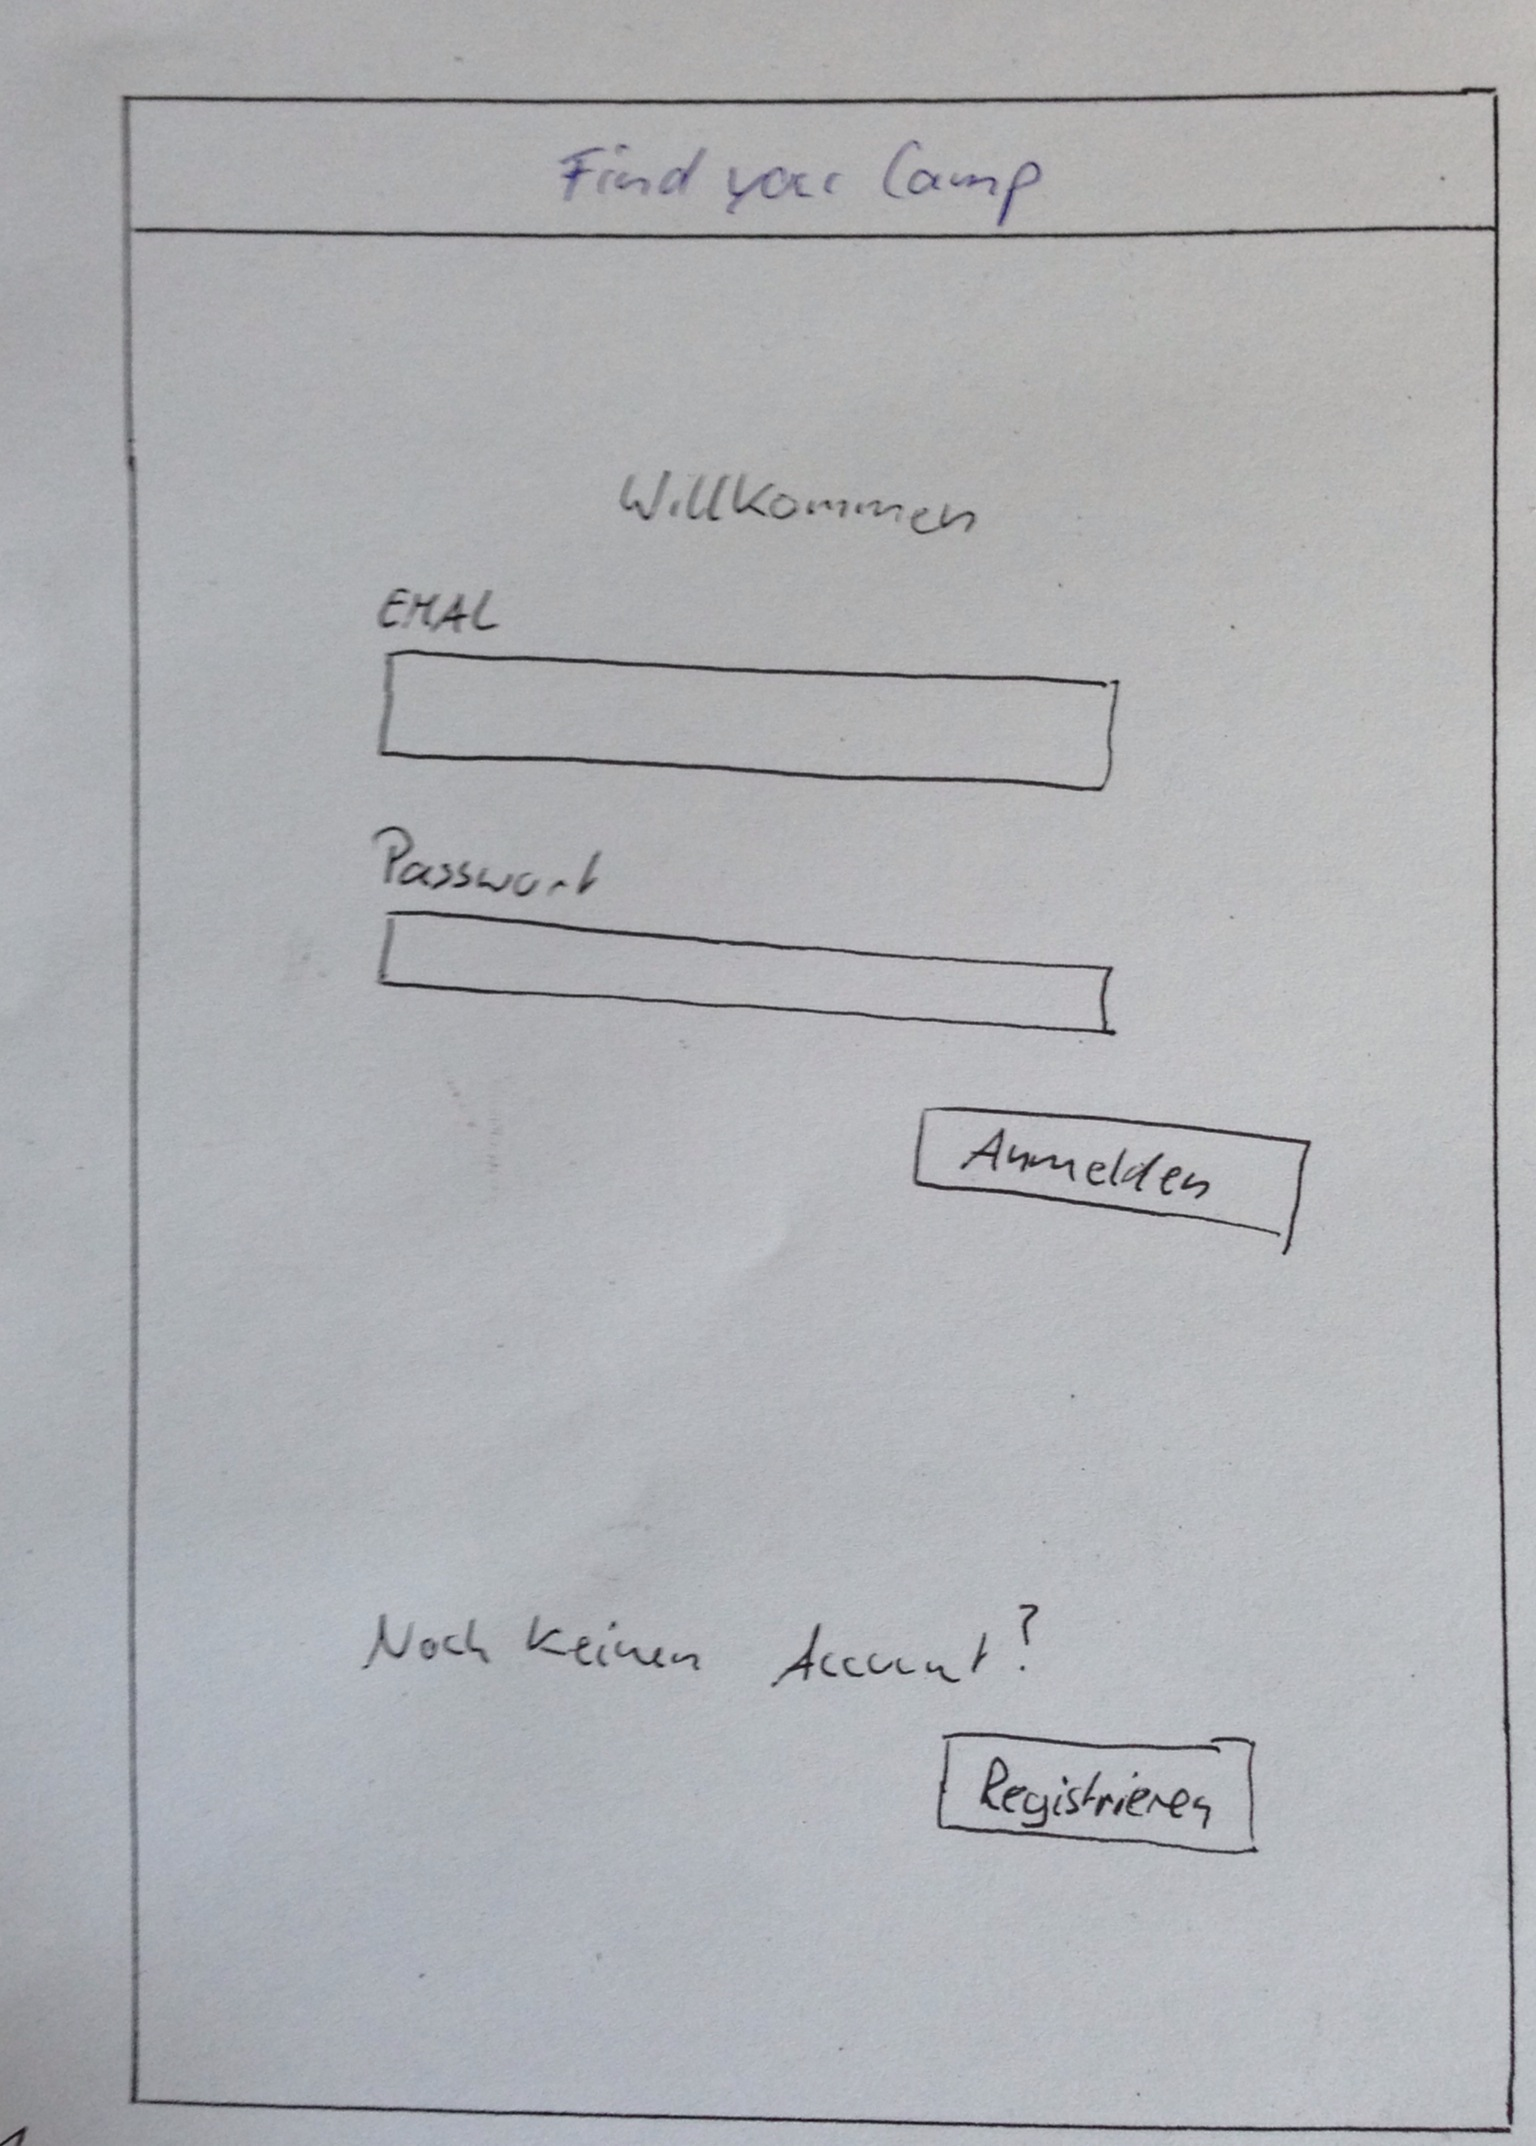
\includegraphics[width=.5\textwidth]{../images/dokulayout/anmelden.jpg}}
\hfill %
\caption{GUI Layout Skizzen: Startauswahl und Einloggen }
\label{gui-skizzen-start-login}
\end{figure}




\newpage

Entscheidet man sich für die Auswahl \textit{Registrieren} wird ein neuer Account angelegt. Auf der ersten Seite (Abb. 3.4a) werden die Grundinformationen eingegeben, wobei hier nur Username und Passwort und Name notwendig sind und die zusätzlichen Informationen jederzeit ergänzt werden können. Nach Eingabe und Kontrolle folgt der zweite Teil der Registrierung, die Auswahl der Genreprioritäten (Abb. 3.4b). Da der Serientracker die Option anbietet, Informationen zu Serien eines bestimtmen Genres zu erhalten, dient dieser Schritt dazu bestimmte Genres zu abonnieren. Auch hier soll die Auswahl später geändert werden können.\\

\begin{figure}[h!]
\centering
\hfill
\subfloat[Registrieren \label{pic:registrieren}]{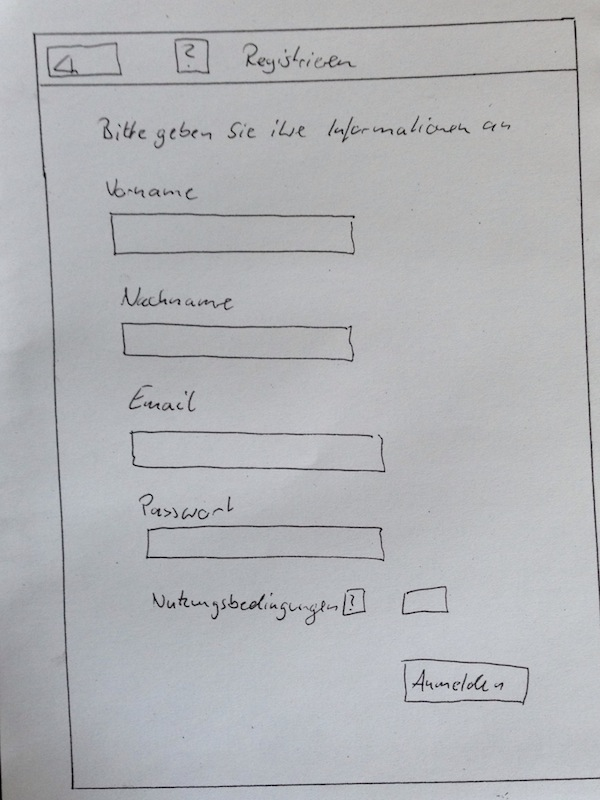
\includegraphics[width=.5\textwidth]{../images/dokulayout/registrieren.jpg}}
\hfill % alternativ auch \hspace{1cm} für genaue Angaben
\subfloat[Prioritäten \label{pic:prioritaeten}]{\includegraphics[width=.5\textwidth]{../images/dokulayout/prioritaeten.jpg}}
\hfill %
\caption{GUI Layout Skizzen: Registrierung }
\label{gui-skizzen-registrierung}
\end{figure}

\vspace{0.2cm}

\begin{wrapfigure}{r}{0cm}
\centering
\includegraphics[width=.5\textwidth]{../images/dokulayout/home.jpg}
\caption{GUI Skizzen: Homeansicht}
\end{wrapfigure}

Nach erfolgreicher Identifizierung des Users folgt der Homebereich (Abb. 3.5). Dies ist der eigentliche Ausgangspunkt für alle Aktivitäten und dient als Benutzerzentrale. Am oberen Bereich findet sich eine statische Menüleiste, die sich in diesem Aufbau durch alle weiteren Bereiche zieht und jederzeit zugänglich ist. Information zum angemeldeten User und die Optionen \textit{Home}, \textit{Favoriten}, \textit{Einstellung}und\textit {Logout}. Home führt jederzeite zur Hauptübersicht, Einstellung ermöglicht entsprechende Möglichkeiten zur Accountverwaltung und Logout meldet den aktuellen Benutzer ab und führt wieder zur Anmeldung. Die Option Favoriten war als Verwaltung zu den angelegten Lieblingsgenre geplant, wurde aber in weiteren Entwürfen in die Einstellungen mit eingebunden, da bis auf eine einfache Auswahl kein größerer Nutzen für den User angeboten wird. Für den Fall das Adminrechte vorhanden sind, wurde in einem späteren Entwurf der zusätzliche Menüpunkt \textit{Hinzufügen} eingebunden. Dort lassen sich neue Serien, Staffeln, Episoden und Genrelisten anlegen. \\


Da im Mittelpunkt des Konzeptes die Benachrichtigung über neue Episoden steht, werden dem User bereits nach einloggen die wichtigsten Informationen präsentiert. Neben einer Suche, werden die Ausstrahlungszeitpunkte der nächsten Episoden angezeigt. Neben dieser Übersicht sollten zudem direkte Benachrichtigungen in Form von Pop-Ups stattfinden, weshalb diese Ansicht vorallem der Erinnerung und Verwaltung dient. Inwiefern eine Darstellung der heutigen Serien in Form eines Kalender realisierbar wäre ist zur Zeit der Konzipierung noch unklar, sollte aber eher als \textit{nice-to-have Feature} betrachtet werden.\\
Dazu gab es die Überlegung Serienempfehlung zu geben, basiernd auf abonnierten Genres. Buttons zu \textit{Meine Serien} und \textit{Meine Listen} führen zu entsprechenden Unterkategoerien.
Meine Serien zeigt einer Auflistung der Serien über die man Benachrichtigungen erhalten möchte und die derzeit angeschaut werden. Meine Listen gibt einen Überblick über angelegte Listen zur Ordnung von Serien nach bestimmten Themen und bietet zudem die Möglichkeit eine neue Liste anzulegen. \\

\parskip 12pt
\parindent 0pt

Nach Auswahl einer bestimmten Serie werden vorhandene Information präsentiert. Allgemeine Informationen, eine Übersicht zu vorhandenen Staffeln und eine Darstellung der nächsten Episode die Ausgestrahlt wird und gegebenfalls die Episode die der Benuter zuletzt gesehen hat. Hierbei würde die Verwaltung mit Hilfe der Seen List stattfinden, wobei auch hier die letztendliche Umsetzung eher unwahrscheinlich ist.
Auf dieser Seite (Abb. 3.6a) kann die Serie einer bestimmten Liste hinzugefügt werden und wird damit abonniert. In einer weiteren Variante der Serienseite (Abb. 3.6b) handelt es sich um die Darstellung unter Adminrechte, wobei die \textit{Add to List} Option nun zum Editieren dieser Seite führt und auch neben den Serien eine entsprechende Editierfunktion eingeführt wird.

\begin{figure} [h!]
\centering
\hfill %
\subfloat[Serienseite User \label{pic:serie}]{\includegraphics[width=.5\textwidth]{../images/dokulayout/serie.jpg}}
\hfill % alternativ auch \hspace{1cm} für genaue Angaben
\subfloat[Serienseite Admin \label{pic:serie2}]{\includegraphics[width=.5\textwidth]{../images/dokulayout/serie2.jpg}}
\hfill %
\caption{GUI Layout Skizzen: Serienübersicht }
\label{gui-skizzen-serien}
\end{figure}


\newpage

Die jeweilige Seasonseite (Abb. 3.7a) zeigt eine Vorschau zu vorhandenen Episoden und bietet dem Admin erneut die \textit{Add Episode} Funktion (Abb. 3.7b). In welcher Form die Episoden aufgeführt werden ist zu diesem Zeitpunkt noch nicht festgelegt und wird bei entsprechender Umsetzung entschieden. Wird eine neue Episode angelegt (Abb. 3.7b) wird entsprechende Serie und Staffel referenziert und die einzelnrn Informationen eingegeben.\\
\begin{figure} [h!]
\centering
\hfill %
\subfloat[Seasonseite \label{pic:staffel}]{\includegraphics[width=.5\textwidth]{../images/dokulayout/staffel.jpg}}
\hfill % alternativ auch \hspace{1cm} für genaue Angaben
\subfloat[Episode anlegen \label{pic:episodeanlegen}]{\includegraphics[width=.5\textwidth]{../images/dokulayout/anlegen.jpg}}
\hfill %
\caption{GUI Layout Skizzen: Seasonübersicht und Verwaltung }
\label{gui-skizzen-season-verwaltung}
\end{figure}

Bei der Planung der GUI, wurden die einzelnen Seiten nach entsprechenden Ideen konzipiert und weiterentwickelt. Die vorgestellten Entwürfe sollten einen kurzen Einblick in die Planungsphase geben und dienten in dieser Form keiner finalen Vorlage, nach der die Entwicklung stattfindet. Aus diesem Grund wird hier im weiteren nicht auf jede einzelne Unterseite eingegangen.\\ Während bei den ersten Varianten vorallem der mögliche Aufbau und die Darstellung der einzelnen Elemente im Vordergrund stand, wurden in späteren Versionen speziell auf entsprechende Funktionalität und Verweisen geachtet. Dabei entstand unter anderem die Adminansicht, welche die Kategorien um verwaltende Optionen erweitert. Ob jede Vorstellung realisierbar bzw. im Projektkontext notwendig ist und wie sich entsprechendes Layout letztendlich entwickelt hat, wird in der Umsetzung dargestellt.\\

\newpage
\subsection{Umsetzung}

Da im Voraus schon auf eine ordentliche Projektstruktur und dementsprechend wiederverwertbare Klassen gesetzt vorhanden waren, konnten diese für den User-Client wieder genutzt werden.\\

Für die GUI sollte \textit{Swing} verwendet werden, welches standardmäßig bei der Komponentenpositionierung auf fixe Pixel setzt. Als Alternative stand ein GUI Builder im Raum oder ein ordnentlicher Layoutmanager.\\
Die Wahl fiel dabei auf den Layout Manager namens MigLayout\footnote{\url{http://www.miglayout.com/}}.\\

Das Ziel für den User-Client war in erster Linie die Basisfunktionen verfügbar zu machen. In Bezug auf zuvor erstellte Konzeptskizze, zeigte sich, dass viele Funktionen angedacht wurden, die für die letztendliche Realisierung keine bedeutende Rolle spiele und aus diesem Grund ersetz wurden. Die gesamte Home Seite stellt nun eine funktionale Übersicht über vorhandene Serien dar. Eine Auswahl führt zu einer kurzen Vorschau, die in der Detailansicht dann die Informationen einer Serien mit Staffeln und Episodenvorschau hervorruft. Alle Funktionen wie Listenerstellung oder Übersicht, sowie Episodendetails konnten aus zeitlichen Gründe nicht mehr umgesetzt werden. Dadurch ergaben sich nun bei Abgabe folgende Funktionen, die anhand von GUIScreenshots einen Einblick in die Umsetzung geben sollen:

\begin{itemize}
  \item Registrierung eines neuen Accounts über XMPP und REST API
  \item Anmeldung via XMPP und REST API
  \item Auslesen der Benutzerdaten über REST API
  \item Auslesen von Serien über REST API
  \item Auslesen von Staffeln über REST API
  \item Auslesen von Episoden über REST API
  \item Anlegen einer neuen Serie über REST API
  \item Abonnieren einer Serie über XMPP PubSub Extension
  \item Empfangen von Notifcations über XMPP PubSub Extension
\end{itemize}



\begin{figure}[H]
  \centering
\includegraphics[width=0.5\textwidth]{../images/screenshots/client-login.png}
\caption{Anmeldung via XMPP und REST API}
\label{login}
\end{figure}

\begin{figure}[H]
  \centering
\includegraphics[width=0.5\textwidth]{../images/screenshots/client-user-settings.png}
\caption{Auslesen der Benutzerdaten über REST API}
\label{settings}
\end{figure}

 \begin{figure}[H]
   \centering
\includegraphics[width=0.7\textwidth]{../images/screenshots/client-series-overview.png}
\caption{Auslesen von Serien über REST API}
\label{overview}
\end{figure}

\begin{figure}[H]
  \centering
\includegraphics[width=0.7\textwidth]{../images/screenshots/client-series-details.png}
\caption{Auslesen von Staffeln und Episoden über REST API}
\label{details}
\end{figure}

\begin{figure}[H]
\includegraphics[width=1\textwidth]{../images/screenshots/client-new-content.png}
\caption{Anlegen einer neuen Serie über REST API}
\label{newcontent}
\end{figure}

\begin{figure}[H]
\includegraphics[width=1\textwidth]{../images/screenshots/client-notification.png}
\caption{Empfangen von Notifcations über XMPP PubSub Extension}
\label{notification}
\end{figure}

\newpage

\subsubsection{Übersicht Packages}

Zum Schluss eine Übersicht der nun vorhanden Packages und deren Funktionen im Zusammenhang mit dem User-Client.


\textbf{de.fhkoeln.gm.serientracker.client}\\
In diesem Paket befindet sich die Main-Klasse für den User-Client.

\textbf{de.fhkoeln.gm.serientracker.client.gui}\\
In diesem Paket befinden sich die Klassen für die Realisierung der GUI für den User-Client.

\textbf{de.fhkoeln.gm.serientracker.client.utils}\\
In diesem Paket befinden sich die mehrer modulare Klassen, die Aufgaben, wie Login, Subscription oder Session-Verwaltung übernehmen.

\textbf{de.fhkoeln.gm.serientracker.jaxb}\\
In diesem Paket befinden sich vom JAXB Generator generierten Objekte.

\textbf{de.fhkoeln.gm.serientracker.utils}\\
In diesem Paket befinden sich zwei Helfer-Klassen, zum einem der Hasher, zum Generieren eines MD5 Hashs sowie der Logger.

\textbf{de.fhkoeln.gm.serientracker.webservice}\\
In diesem Paket befindet sich die Main-Klasse für den REST Server, sowie die Klasse für die Servereinstellungen.

\textbf{de.fhkoeln.gm.serientracker.webservice.data}\\
In diesem Paket befinden sich die Data-Handler für die Ressourcen. Aufgrund des modularen Aufbaus wurden diese aus den Service-Klassen extrahiert. Sie sind das Bindeglied zwischen dem Service und dem File-Handler, siehe utils Paket.

\textbf{de.fhkoeln.gm.serientracker.webservice.resources}\\
In diesem Paket befinden sich die Services für die Ressourcen auf welche über die Clienten zugegriffen wird.

\textbf{de.fhkoeln.gm.serientracker.webservice.utils}\\
In diesem Paket befindt sich eine Helfer-Klasse, dem File-Handler, welche die Verbindung zwischen Dateisystem und JAXB Objekt implementiert.

\textbf{de.fhkoeln.gm.serientracker.xmpp}\\
In diesem Paket befindet sich die Main-Klasse für den XMPP-Debug-Client, sowie die Klasse für die Servereinstellungen.

\textbf{de.fhkoeln.gm.serientracker.xmpp.gui}\\
In diesem Paket befinden sich die Klassen für die Realisierung der GUI für den XMPP-Debug-Client.

\textbf{de.fhkoeln.gm.serientracker.xmpp.utils}\\
In diesem Paket befinden sich die mehrer modulare Klassen, die Aufgaben, wie Verbindungsaufbau oder Subscription-Verwaltung übernehmen.

\textbf{de.fhkoeln.gm.serientracker.bot}\\
In diesem Paket befindet sich die Main-Klasse für den Bot-Client. Siehe hierfür Abschnitt "Zusatz: Bot-Client".

\textbf{de.fhkoeln.gm.serientracker.bot.jobs}\\
In diesem Paket befinden sich die Klassen, die die Jobs übernehmen, wenn der Cronjob das Event ausführt.

\textbf{de.fhkoeln.gm.serientracker.bot.utils}\\
In diesem Paket befindt sich eine Wrapper-Klasse, welche die Verbindung zwischen der Quartz Scheduler API und dem Clienten implementiert.

\newpage

\subsubsection{Zusatz: Bot-Client}

Für das Veröffentlichen von Items, also den Notifications mit der Info über die bevorstehende Episodenaustrahlung, wurde ein Bot Client angelegt.\\
Der Bot-Client übernimmt dabei die Aufgabe pro Serie die Nodes anzulegen. Dazu scannt er die Datenbestand und wird zur jeder Serie drei Nodes anlegen, da ein User selbst entscheiden kann, ob er 5, 10 oder 15 Minute vorher informiert werden möchte. Die Node ID ist dabei im Format \textsf{series:\{Serien ID\}:\{[5|10|15]\}} definiert.\\
Gleichzeitig scannt er den Datenbestand nach den Episoden ab und prüft ob das Austrahlungsdatum in der Zukunft liegt.\\
Liegt es in der Zukunft wird ein Event angelegt. Dazu wurde die Quartz Scheduler Bibliothek\footnote{\url{http://quartz-scheduler.org}} eingesetzt. Mit ihr ist es möglich sogenannte Cronjobs anzulegen. Die beiden entwickleten Jobs \textit{ProfilerJob} und \textit{NotificationJob} übernehmen dabei die Verarbeitung.\\

Aus zeitlichen Gründen konnte  das Senden der automatisieren Notifcations nicht mehr implementiert werden. Zum Testen der Notifcation kann deshalb der XMPP Debug Client genutzt werden.


\newpage


	%Die Zähler für Tabellen und Abbildungen werden zurückgesetzt, damit
	%in jedem Kapitel die Nummerierung neu beginnt
	\setcounter{table}{1}
	\setcounter{figure}{1}
	%Einbinden des zweiten Kapitels
	%!TEX root = ../konzept.tex

\chapter{WBA Systemarchitektur}

%!TEX root = ../konzept.tex

\section{Kommunikationsabläufe und Interaktionen}

TODO Alternativen genauer betrachten

Zur Festlegung der Systemarchitektur werden zunächst die Anforderungen anhand eines möglichen Kommunikationsablaufs eines erfolgreichen Interaktionsszenario in einer klassischen Server-Client-Architektur betrachtet (Abb. \ref{fig:kommunikationsablauf}).\\

Ein potentieller Mieter nutzt unsere Smartphone-Anwendung zunächst um seinen eigenen Standort zu ermitteln. Daraufhin sendet er seine Anfrage an unser Hauptsystem, welches das erste \textit{Matching} durchführt.

In einer Datenbank befinden sich Zuordnungen zwischen Vermieter und dem Ort eines Mietobjektes. Auf Basis dieser Datenmenge wird ein Abgleich zwischen angefragtem Ort und vorhandenen Orten durchhgeführt. Bei allen möglichen Treffern wird der zugehörige Nutzer herausgefiltert.

Zu den relevanten Daten eines Nutzers gehört unter anderem eine Identifikationsnummer, unter welcher das Smartphone des Nutzers ansprechbar ist.
Dadurch werden die nun gefilterten Vermieter angesprochen und bekommen ein Ereignis zugesendet.

Das Ereignis beinhaltet die relevanten Daten der Anfrage durch den Mieter. Sobald das Ereignis das Ziel erreicht hat, wird auf dem Endgerät des Vermieters das zweite \textit{Matching} durchgeführt, denn wie in der Martkanalyse bereits identifiziert wurde, werden direkte Personen- und Objektdaten auf den Endgeräten der Nutzer gespeichert.

Das zweite \textit{Matching} vergleicht das gesendete Profil mit dem auf dem Gerät gespeicherten Profil. Ein Algorithmus berechnet dabei einen Quotienten, welcher den Grad der Übereinstimmung widerspiegelt. Übersteiget dieser Quotient einen Wert X, wird der Vermieter über die Anfrage visuell über die Anfrage benachrichtigt, auf welche dieses reagieren muss.
Der Vermieter kann die Anfrage bestätigen oder ignorieren. Bei einer Bestätigung wird der Mieter über die Bestätigung informiert und kann die Daten des potentiellen Mietobjektes einsehen, sowie weiteren Kontakt zu dem Vermieter aufnehmen.

\begin{figure}[H]
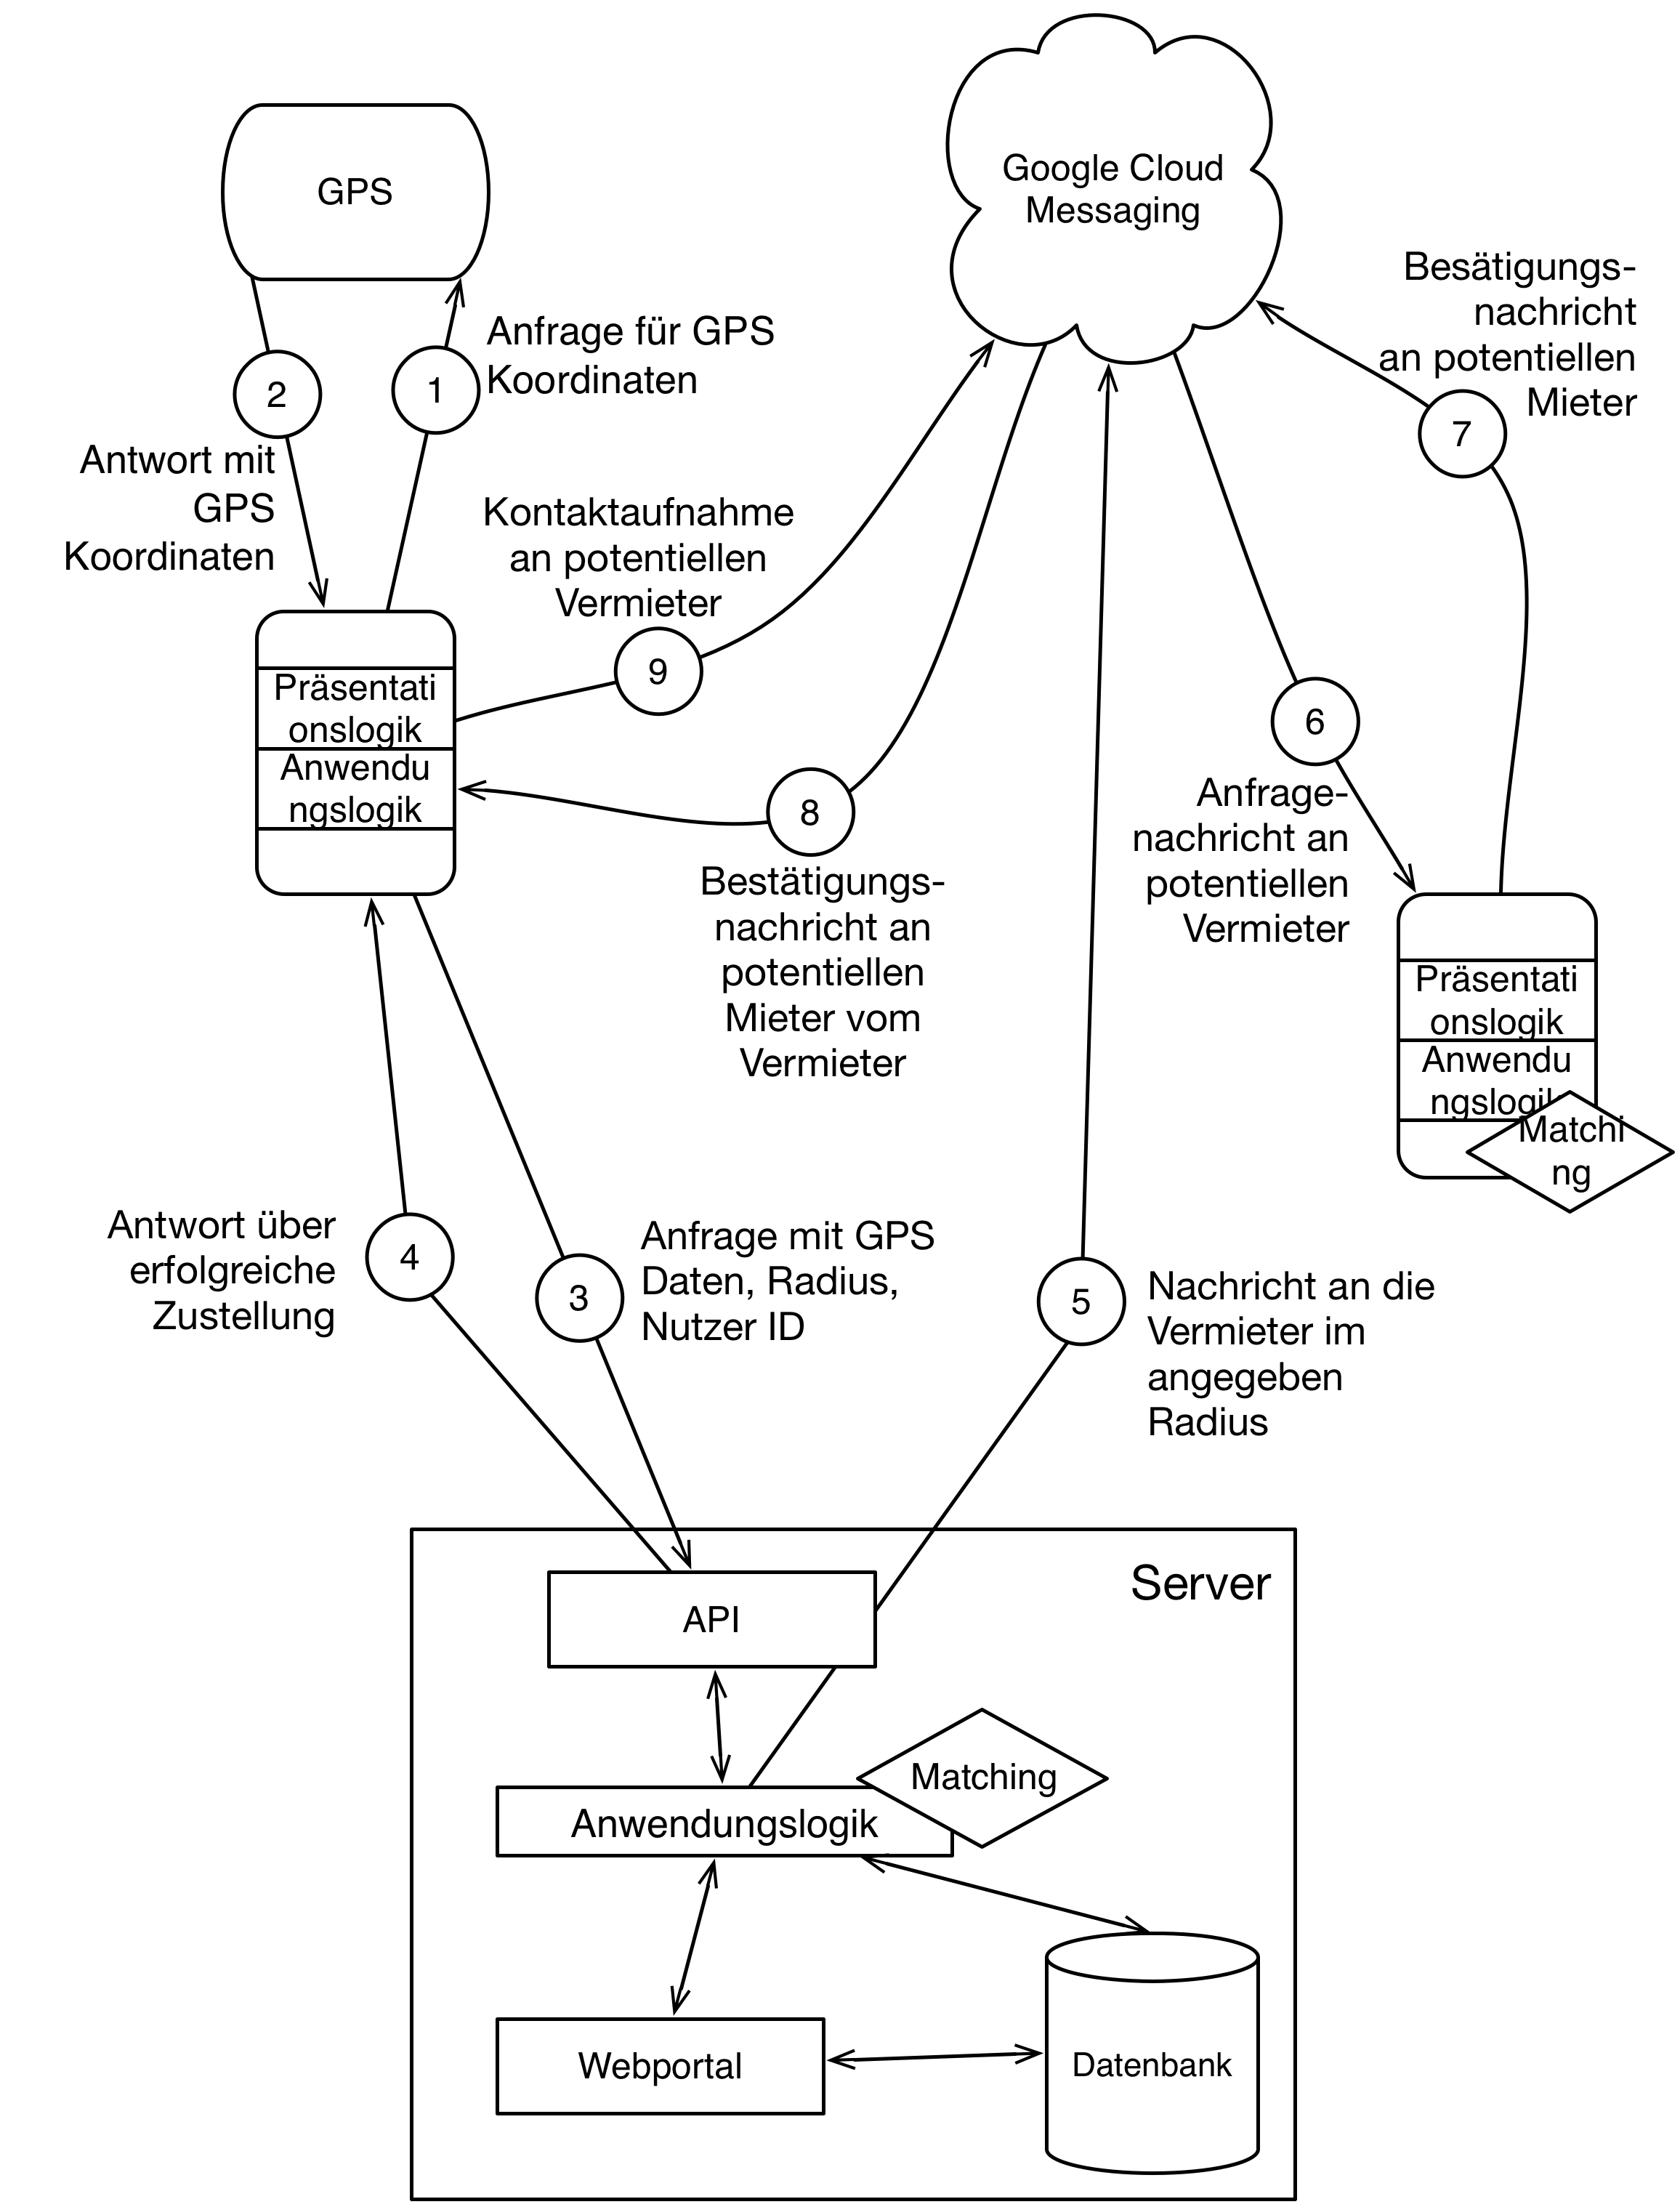
\includegraphics[width=.9\textwidth]{./images/kommunikationsablauf.png}
\caption{Kommunikationsablauf eines erfolgreichen Interaktionsszenario }
\label{fig:kommunikationsablauf}
\end{figure}

Auf Basis dieses Kommunikationsablaufs kann nun auf die einzelnen Komponenten der Systemarchitektur eingegangen werden.



\newpage

%!TEX root = ../konzept.tex

\section{Verteilte Anwendung}



Softwarekomponenten, verteilte Systeme,Kohärenz


Für die Analyse zunächst ein Überblick über die möglichen Architektur-Paradigmen, mit einer ersten Abwägung.\\

\textbf{Publish-Subscribe}\\


Entfernte Prozedur- und Methodenaufrufe => Polling

WS* Architektur


Lose Kopplung


\newpage

%!TEX root = ../konzept.tex

\section{Datenmodell}

Aufgrund der verteilten Anwendung und der lokalen Speicherung von Daten müssen die einzelen Komponten untereinander die Daten austauschen. Dafür ist es nötig, dass jede Kompontene mit den Daten arbeiten kann.


TODO


\newpage

%!TEX root = ../konzept.tex

\section{Datenmodell}



%\newpage

%\input{chapter/kapitel45}


	%Die Zähler für Tabellen und Abbildungen werden zurückgesetzt, damit
	%in jedem Kapitel die Nummerierung neu beginnt
	\setcounter{table}{1}
	\setcounter{figure}{1}
	%Einbinden des zweiten Kapitels
	%!TEX root = ../dokumentation.tex

\chapter{Kapitel 5}




	%Die Zähler für Tabellen und Abbildungen werden zurückgesetzt, damit
	%in jedem Kapitel die Nummerierung neu beginnt
	\setcounter{table}{1}
	\setcounter{figure}{1}
	%Einbinden des zweiten Kapitels
	
	%!TEX root = ../konzept.tex


\chapter{Literatur- und Quellenverzeichnis}

Literaturquellen 
\begin{itemize}
\item
Prof. Dr. Gerhard Hartmann: Draft zum kleinen Handbuch der Mensch-Computer Interaktion, März 2013
\item
Alan Dix: Human-Computer Interaction (3rd Edition), 2003
\item 
David Benyon: Designing Interactive Systems, A comprehensive guide to HCI and interaction Design (2nd Edition) 
\item
ISO 9241-210: Human-centred design for interactive systems nach Draft von Prof. Dr. Hartmann, komplett käuflich zu erwerben unter \\http://www.iso.org/iso/catalogue\_detail.htm?csnumber=52075

\end{itemize}

Internetquellen 
\begin{itemize}
\item
Freagle: http://www.freagle.org/ letztes Sichtdatum 25.10.2013
\item
Campinmygarden: http://campinmygarden.com// letztes Sichtdatum 25.10.2013
\item
ADAC App: http://www.adac.de/produkte/buecher\_magazine/camping-stellplatz-app-iphone-android/ letztes Sichtdatum 25.10.2013
\item
Couchsurfing: www.couchsurfing.org letztes Sichtdatum 25.10.2013
\item
Coouchsurfing: http://en.wikipedia.org/wiki/CouchSurfing letzes Sichtdatum 25.10.2013
\item
Abb.2.1: http://upload.wikimedia.org/wikipedia/commons/6/6d/Couchsurfers\_by\_country.png
\item
Airbnb: www.airbnb.de letztes Sichtdatum 25.10.2013
\item
Sharing Umfrage: http://de.scribd.com/doc/38788695/The-New-Sharing-Economy-Study-Report-by-Latitude-and-Shareable-Magazine letztes Sichtdatum 25.10.2013
\item
Abb.3.1: http://blog.procontext.com/images/posts2010/prozessergebnisse-des-usability-engineering-1200x900.png
\item
Gewerbe: http://www.gewerbe-anmelden.info/gewerbeanmeldung.html letztes Sichtdatum 27.10.2013
\item
Gewerbe: http://portal.wko.at/wk/format\_detail.wk?angid=1\&stid=420794\&dstid=0 letztes Sichtdatum 27.10.2013
\item
Gewerbe: http://www.steuerberaten.de/tag/nebengewerbe/ letztes Sichtdatum 27.10.2013
\item
Grunddlegenede Publikationen zum Usage centered Design \\http://www.foruse.com/questions/index.htm\#13 letztes Sichtdatum 27.10.2013


\end{itemize}

\newpage
 

	%Die Zähler für Tabellen und Abbildungen werden zurückgesetzt, damit
	%in jedem Kapitel die Nummerierung neu beginnt
	\setcounter{table}{1}
	\setcounter{figure}{1}
	%Einbinden des zweiten Kapitels
	
	%%!TEX root = ../Dokumentation.tex

\chapter{Autorenübersicht}

\begin{table}[H]

\centering
\begin{tabular}{l c c}
\\ [-0.5ex]
\hline\hline
\\ [-0.5ex]
Themenbereich & Dennis Meyer & Dominik Schilling
\\ [1.5ex]
\hline
\\ [-0.5ex]
Konzept & 50\% & 50\% \\[1ex]
Projektbezogene XML Schemata & 70\% & 30\% \\[1ex]
Ressourcen und Semantik der HTTP - Operationen & 50\% & 50\% \\[1ex]
RESTful Webservice & 40\% & 60\% \\[1ex]
XMPP Konzeption & 40\% & 60\%\\[1ex]
XMPP Cliententwicklung & 30\% & 70\%\\[1ex]
Client & 50\% & 50\% \\[1ex]
\hline
\end{tabular}
\label{tab:autoren}
\end{table}
 

%Zeilenabstand 1 fach für die Verzeichnisse
\singlespacing
%Einbindne der Verzeichnisse
%!TEX root = ../Dokumentation.tex

  %Erzeugt ein Abbildungsverzeichnis
	\listoffigures
	%Fügt die Zeile "`Abbildungsverzeichnis"' als Chapter ins Inhaltsverzeichnis ein
	\addcontentsline{toc}{chapter}{Abbildungsverzeichnis}

	%Erzeugt ein Tabellenverzeichnis
	\listoftables
	%Fügt die Zeile "`Tabellenverzeichnis"' als Chapter ins Inhaltsverzeichnis ein
	\addcontentsline{toc}{chapter}{Tabellenverzeichnis}

	%Erzeugt ein Codeverzeichnis
	\lstlistoflistings
	%Fügt die Zeile "`Codeverzeichnis"' als Chapter ins Inhaltsverzeichnis ein
	\addcontentsline{toc}{chapter}{Codeverzeichnis}

	%Erzeugt ein Glossar
%	\printnomenclature
	%Fügt die Zeile "`Glossar"' als Chapter ins Inhaltsverzeichnis ein
%	\addcontentsline{toc}{chapter}{Glossar}

	%Ändert den Stil des Literaturverzeichnisses
	\bibliographystyle{geralpha}
	%Erzeugt das Literaturverzeichnis anhand der Datei "`literatur.bib"'
%	\bibliography{doc/literatur}
	%Fügt die Zeile "`Literaturverzeichnis"' als Chapter ins Inhaltsverzeichnis ein
%	\addcontentsline{toc}{chapter}{Literaturverzeichnis}


%Zeilenabstand 1,5 fach für den Eid
\onehalfspacing
%Einbinden des Eides
%%!TEX root = ../konzept.tex

\chapter*{Eidesstattliche Erklärung}
\addcontentsline{toc}{chapter}{Eidesstattliche Erklärung}
Ich versichere, die von mir vorgelegte Arbeit selbständig verfasst zu haben.\\ \\
Alle Stellen, die wörtlich oder sinngemäß aus veröffentlichten oder nicht veröffentlichten Arbeiten anderer entnommen sind, habe ich als entnommen kenntlich gemacht. Sämtliche Quellen und Hilfsmittel, die ich für die Arbeit benutzt habe, sind angegeben.\\ \\
Die Arbeit hat mit gleichem Inhalt bzw. in wesentlichen Teilen noch keiner anderen Prüfungsgbehörde vorgelegen.
\vspace{1.5cm}
\\
Gummersbach, 28. Oktober 2013
\vspace{3cm}
\\
Dennis Meyer \\
Dominik Schilling


\end{document}
